%%%% Version 8 (compressed, 2026-08-26). Reframed revision of main_v7.tex; no new experiments,
%%%% every number is the number that stood in v7, traced to the same artifacts.
%%%%
%%%% Framing (Kye's instructions, 2026-08-25): claims generalised to a stage-by-stage analysis
%%%% of a biosignal pipeline with EMG jaw activity as the case study; new title; Background
%%%% 2.4 "Where this study stands" + Table 1 (positioning, facts checked against sources
%%%% 2026-08-25); Methods 3.1 "Why the data were collected for this study" (repository check
%%%% PhysioNet / Zenodo / Mendeley Data, 2026-08-25); Discussion 5.3 "What transfers beyond
%%%% this case study"; protocol corrected to 60-s recordings (v7 said 3-minute trials);
%%%% cites refs_v8.bib (two corrected entries, fifteen additions; refs.bib untouched).
%%%%
%%%% Compression (Kye's instructions, 2026-08-26): body cut from 29 pp to a 20-pp target
%%%% before the references (achieved: references begin on p. 20 of 26) without removing any
%%%% table or figure except the study-overview
%%%% figure (former Fig. 1, Figures/study_pipeline.pdf) and the sample-flow panel (former
%%%% Fig. 2b, Figures/v5/sample_flow.png), both removed at Kye's request. Cuts are to prose,
%%%% captions and table notes; technical detail that did not carry a contribution, the
%%%% problem statement or an insight was trimmed. Figure widths reduced modestly. The
%%%% uncompressed v8 text (34 pp) is kept beside this file as main_v8_long.tex.bak.
%%%%
%%%% Artifact references (unchanged):
%%%%   outputs/runs/modality_and_no_chewing_20260810T020642_cead62e4  (emg_only conditions)
%%%%   outputs/runs/baselines_emg_only_20260816                      (RQ3 architectures)
%%%%   outputs/screening/emg_only_filter_contrast.json                (RQ1 filter contrast)
%%%%   outputs/screening/emg_only_design.json                         (RQ4 design constraints)
%%%%   outputs/screening/emg_only_contrast.json                       (RQ3 feature baselines)
%%%%   outputs/data_audit/7ebbcc8d74c0bbe0/                           (guards, sweeps, mains)
%%%%   outputs/benchmarks/benchmark_emg_only.json                     (parameters, latencies)
%%%% Run-dependent figures live in Figures/v5/ so that main_4.tex still compiles.
\documentclass[pdflatex,sn-nature,iicol]{sn-jnl}

\usepackage{graphicx}
\usepackage{multirow}
\usepackage{amsmath,amssymb}
\usepackage{booktabs}
\usepackage{mathrsfs}
\usepackage[title]{appendix}
\usepackage{xcolor}
\usepackage{textcomp}
\usepackage{manyfoot}
\usepackage{indentfirst}

\graphicspath{{./}{figures/}{Figures/}}

%%%% Float packing. These change typesetting only, and add or remove no content.
%%%% The default LaTeX fractions reserve so much of each page for text that a document
%%%% with eleven full-width floats strands roughly two pages in placement dead space.
\renewcommand{\topfraction}{0.92}
\renewcommand{\bottomfraction}{0.70}
\renewcommand{\textfraction}{0.06}
\renewcommand{\floatpagefraction}{0.80}
\renewcommand{\dbltopfraction}{0.92}
\renewcommand{\dblfloatpagefraction}{0.80}
\setcounter{topnumber}{3}
\setcounter{bottomnumber}{2}
\setcounter{totalnumber}{4}
\setcounter{dbltopnumber}{3}
\setlength{\floatsep}{6pt plus 2pt minus 2pt}
\setlength{\textfloatsep}{8pt plus 2pt minus 2pt}
\setlength{\dblfloatsep}{6pt plus 2pt minus 2pt}
\setlength{\dbltextfloatsep}{8pt plus 2pt minus 2pt}
\setlength{\intextsep}{6pt plus 2pt minus 2pt}

\begin{document}

\title[Where Does the Performance Come From?]{Where Does the Performance Come From? A Stage-by-Stage Analysis of a Surface-EMG Jaw-Activity Classification problem}

\author[1]{\fnm{Mohammad Hassan} \sur{Farhadi}}
\author[1]{\fnm{Ali} \sur{Rabiee}}
\author[1]{\fnm{Rahul} \sur{Singh}}
\author[2,3]{\fnm{Mariusz P.} \sur{Furmanek}}
\author*[1]{\fnm{Reza} \sur{Abiri}}\email{reza\_abiri@uri.edu}
\author*[4]{\fnm{Theodore A.} \sur{Walls}}\email{walls@uri.edu}

\affil[1]{\orgdiv{Department of Electrical, Computer, and Biomedical Engineering}, \orgname{University of Rhode Island}, \orgaddress{\city{Kingston}, \state{RI}, \country{United States}}}
\affil[2]{\orgdiv{Department of Physical Therapy}, \orgname{University of Rhode Island}, \orgaddress{\city{Kingston}, \state{RI}, \country{United States}}}
\affil[3]{\orgdiv{Institute of Sport Sciences, Academy of Physical Education in Katowice}, \orgaddress{\city{Katowice}, \country{Poland}}}
\affil[4]{\orgdiv{Department of Psychology}, \orgname{University of Rhode Island}, \orgaddress{\city{Kingston}, \state{RI}, \country{United States}}}

\abstract{Classification pipelines for physiological signals are reported almost entirely through summary accuracies, which say how well a pipeline scored and little about which of its stages earned the score. This paper is a systematic, stage-by-stage analysis of one such pipeline, in a case study controlled from the participant's chair to the decision: classifying quiet rest and four instructed jaw activities from surface electromyography (EMG), a problem relevant to bruxism. The data, 100 laboratory recordings from five adults with a prior clinical diagnosis of bruxism, were collected for the purpose, because no public dataset offers continuous masticatory-muscle recordings archived as acquired with a synchronised task marker and a quiet-rest condition. On unseen participants the pipeline separated the five conditions at 81.7\% accuracy, 72.0\% macro-F1 and a macro ROC--AUC of 0.958. Pricing its stages on identical windows, folds and labels gave a consistent ordering. Signal quality set a ceiling: the acquisition hardware had already removed the 60-Hz mains fundamental and the surviving interference was harmonic, so the conventional single-notch chain removed the one frequency that was absent, and correcting it gained 29.3 points of macro-F1. Above that ceiling, what a model could represent mattered more than how large it was, and two choices fixed before any model was trained, temporal context and normalisation scope, were each worth as much as the architecture or more. The magnitudes belong to this cohort and laboratory; what transfers is the procedure, which applies to EEG, ECG or inertial pipelines as readily as to EMG: audit the signal against what the analysis assumes, publish a measured interference statistic beside every accuracy, and price the choices made before modelling against the model itself.}

\keywords{Biosignal classification, Signal-processing pipeline, Performance attribution, Surface electromyography, Jaw-activity classification, Bruxism, Wavelet decomposition, Convolutional neural networks, Signal-quality audit, Leave-one-subject-out validation, Data collection protocol}

\maketitle
\section{Introduction}

A classifier for physiological signals is the last stage of a long pipeline. Before a window of signal reaches a model it has passed through a sensor and its placement, an amplifier with filters of its own, an offline filter chain, a segmentation rule, a normalisation scope and an evaluation protocol, and each of those stages can move the reported number by more than the model does. Yet pipelines are reported, in electromyography (EMG) as in electroencephalography (EEG), electrocardiography and inertial sensing, almost entirely through a final accuracy and a block diagram~\cite{thymi2021signal,roy2019deep,lipton2019troubling}. Reviews of deep learning on EEG find preprocessing and validation reported inconsistently~\cite{roy2019deep}, the value of preprocessing itself is contested~\cite{delorme2023eeg}, the variance from seeds and data splits is often larger than the gains papers claim~\cite{bouthillier2021accounting}, and reporting standards now ask for the attribution that a single accuracy cannot supply~\cite{kapoor2024reforms,collins2024tripod}.

This paper is a systematic, stage-by-stage analysis of one such pipeline. We chose a case study we could control from the participant's chair to the decision, built the pipeline end to end, and then priced it: each stage is varied while everything else is held fixed, on the same windows, folds and labels, and the effects are placed on one scale. The pipeline is ordinary in its parts: validate the signal, decompose it into frequency bands with a wavelet transform, classify each window with a small convolutional network, and evaluate under a nested leave-one-subject-out (LOSO) protocol in which nothing fitted during training has seen the participant being scored. What is unusual is that every part reports what it was worth.

The case study is the classification of jaw activity from surface EMG. Bruxism, the habitual clenching or grinding of the teeth, is common, wears down teeth and loads the jaw joint, and is difficult to observe directly because it happens during sleep or while people are awake and not attending to it~\cite{lavigne2008bruxism,manfredini2013epidemiology,melo2019bruxism,wetselaar2019prevalence}. Sleep bruxism has a demanding reference standard, overnight polysomnography with audio and video~\cite{lavigne1996sleep}; awake bruxism has no instrumental standard at all~\cite{bracci2018frequency,zani2019ecological}. Surface EMG records the jaw-closing muscles directly~\cite{raez2006techniques,colonna2023electromyographic,thymi2021signal}, but clenching, grinding and chewing all contract the same masseter and temporalis muscles, and separating them on a person the system has never encountered is a hard problem, one on which many groups have reported good accuracies without an account of where the accuracy came from~\cite{sonmezocak2021detection,gul2024advanced,ishtiaq2025wearable,heyat2020computational}.

A stage-by-stage analysis also needs data that allow the stages to be varied: continuous recordings archived as acquired, with a record of what the hardware did to them, a synchronised task marker, a quiet-rest condition and more than one food. No public dataset offers that combination (Section~\ref{sec:why_data}), so the recordings were collected for this study: 100 laboratory recordings from five adults with a prior clinical diagnosis of bruxism, covering quiet rest and four instructed jaw activities.

The answer has a shape worth stating up front. Signal quality sets a ceiling, and no modelling choice reaches above it. Below that ceiling, what a model can represent matters more than how many parameters it has: the largest model we evaluated placed third of four and the smallest placed second. Choices made before any model was trained, such as how long an analysis window is allowed to be, were worth as much as the architecture or more.

\paragraph{Scope.} International consensus defines bruxism as masticatory-muscle activity that may involve clenching or grinding with tooth contact, or bracing and thrusting without it, in sleep or awake~\cite{lobbezoo2013bruxism,lobbezoo2018international,verhoeff2025definitions,manfredini2022bruxism}; tooth contact is neither necessary for all bruxism activities nor sufficient to establish that an activity is bruxism. Every activity analysed here was performed on instruction in a laboratory: the class names rest, movement, clenching, grinding and chewing denote experimental conditions, and a classifier that separates them is not a diagnostic device~\cite{manfredini2024standardised}.

\paragraph{Research questions.} Four questions are posed for the case study. Each can be asked of any biosignal pipeline, and the last two rarely are.

\textbf{RQ1.} How much of what a classifier learns from these recordings comes from the participants' physiology, and how much from mains interference? Two filter chains are run over identical windows, folds and labels, so the filter is the only thing that differs.

\textbf{RQ2.} Can four channels of surface EMG separate quiet rest from four instructed jaw activities on a participant the system has never seen?

\textbf{RQ3.} Which part of the model does the work: the wavelet representation, the architecture built on it, or simply the number of parameters?

\textbf{RQ4.} How do those modelling choices compare against choices fixed before any model was trained: the analysis window length, the temporal context available to a decision, and the scope over which the signal is normalised?

\paragraph{Contributions.} First, a stage-by-stage analysis in which signal quality, learned representation, architecture, temporal context and normalisation scope are priced on one comparable scale, on identical windows and folds, giving a measured budget (Table~\ref{tab:budget}) of a kind this application area has not had. Second, a purpose-built protocol and dataset, five conditions including quiet rest and three foods recorded from bilateral masseter and temporalis pairs with a synchronised marker and archived raw, with the reasons an existing dataset could not have served (Section~\ref{sec:why_data}). Third, a five-class result on unseen participants that includes a quiet-rest class, which activity-only designs omit and which is what makes a false-alarm estimate possible. Fourth, a pipeline in which every reported number is regenerated from a saved prediction ledger. Fifth, two inexpensive checks other groups can adopt directly: drawing the filter response over the measured spectrum of the recordings, and fingerprinting every channel of every recording before fitting anything to it.

\section{Background}


\begin{table*}[h]
  \centering
  \caption{Where this study stands. Machine-learning studies of jaw activity and bruxism, and the alternative sensing routes, on the axes that determine what a reported accuracy means. ``Held-out participants'' states whether every test participant was absent from training; ``Varied'' lists what each study compared within itself. ``n.s.'': not stated in the source.}
  \label{tab:positioning}
  \footnotesize
  \begin{tabular*}{\textwidth}{@{\extracolsep{\fill}}p{0.13\textwidth}p{0.12\textwidth}p{0.11\textwidth}p{0.16\textwidth}p{0.12\textwidth}p{0.13\textwidth}p{0.07\textwidth}@{}}
    \toprule
    Study & Signal & Cohort & Conditions & Held-out participants & Varied & Data \\
    \midrule
    \multicolumn{7}{l}{\emph{Masticatory-muscle surface EMG}}\\
    Sonmezocak \& Kurt 2021~\cite{sonmezocak2021detection} & masseter sEMG & 10 volunteers & relaxed, clenching, rhythmic grinding, fatigue or pain; instructed & no: random split of segments & features, network settings & n.s. \\
    Gul et al.\ 2024~\cite{gul2024advanced} & bilateral temporalis and masseter sEMG & 10 healthy volunteers, simulating & rest, talking, chewing, clenching, grinding; three postures & no: 10-fold over windows, oversampled & classifier, muscle, posture & on request \\
    Ishtiaq et al.\ 2025~\cite{ishtiaq2025wearable} & temporalis and masseter sEMG, wearable & 30 volunteers, 5 trials each & clenching vs.\ other; supine & n.s.; oversampled & classifier, oversampling & n.s. \\
    Zhang \& Amft 2018~\cite{zhang2018monitoring} & temporalis sEMG in eyeglasses & 10 volunteers & chewing and eating vs.\ other; laboratory and 122~h free living & n.s. & setting, food hardness & n.s. \\
    Castroflorio et al.\ 2013, 2014~\cite{castroflorio2013use,castroflorio2014detection} & masseter sEMG and ECG holter, at home & 21 bruxers, 21 controls & sleep-bruxism episodes against polysomnography & per-participant agreement; rule-based & device vs.\ reference & n.s. \\
    \midrule
    \multicolumn{7}{l}{\emph{Other signals}}\\
    Heyat et al.\ 2020; Tripathi et al.\ 2024~\cite{heyat2020computational,tripathi2024computational} & overnight PSG: EEG, ECG, chin EMG & public database; 2 bruxism subjects available & bruxism vs.\ healthy; sleep stages & no: segment-level cross-validation & channel, classifier ensemble & public \\
    Martinot et al.\ 2021~\cite{martinot2021artificial} & mandibular movement, chin sensor & 67 suspected-OSA patients & phasic sleep bruxism against polysomnography & n.s. & device vs.\ reference & n.s. \\
    Bondareva et al.\ 2021~\cite{bondareva2021earables} & in-ear inertial unit & 13 volunteers & grinding, clenching vs.\ silent; still and while moving & yes: leave-one-out & sensor, classifier & n.s. \\
    Schlaepfer et al.\ 2026~\cite{schlaepfer2026new} & chin inertial unit & 3 volunteers, 21 recordings & grinding, opening and closing, other; simulated & no: pooled 80/20 split & classifier, sensor subset & on request \\
    Shen et al.\ 2026~\cite{shen2026bruxism} & 60-GHz radar & 3 volunteers, 180 clips & grinding vs.\ none & no: 10-fold over clips & classifier & n.s. \\
    \midrule
    \textbf{This study} & bilateral temporalis and masseter sEMG, 4 channels, archived as acquired with metadata & 5 adults with a prior clinical diagnosis & rest, movement, clenching, grinding, chewing of three foods; awake, instructed & \textbf{yes}: nested LOSO, 3 seeds & \textbf{signal chain, representation, architecture, window and context, normalisation scope} & on request \\
    \bottomrule
  \end{tabular*}
\end{table*}


\subsection{EMG-based assessment of masticatory activity}

Surface EMG is widely used for ambulatory assessment because it measures masticatory activation directly~\cite{raez2006techniques,farella2008masticatory}. Polysomnography with audio and video remains the reference standard for sleep bruxism~\cite{lavigne1996sleep,stuginski2016detection}, and portable instruments show variable agreement with it~\cite{casett2017validity,cidverdejo2024instrumental}. Castroflorio et al.~\cite{castroflorio2013use,castroflorio2014detection} combined EMG and electrocardiographic information to identify sleep-bruxism episodes at home; multi-day home recording is feasible~\cite{colonna2023electromyographic}, and consensus guidance exists for ambulatory EMG~\cite{lobbezoo2020consensus}.

Machine-learning studies report high performance on controlled tasks, although labels, participants and validation protocols differ. Sonmezocak and Kurt~\cite{sonmezocak2021detection,sonmezocak2021machine} reported greater than 90\% accuracy from masseter-EMG features across relaxation, clenching, rhythmic grinding and fatigue or pain; Gul et al.~\cite{gul2024advanced} evaluated simulated sleep-bruxism activity across postures, Ishtiaq et al.~\cite{ishtiaq2025wearable} clenching detection from a two-muscle wearable, and Heyat et al.~\cite{heyat2020computational} and Tripathi et al.~\cite{tripathi2024computational} bruxism from public polysomnographic EEG and ECG; Lan et al.~\cite{lan2022comparative} described different surface-EMG patterns during centric and eccentric activities. Other sensing routes include mandibular movement~\cite{martinot2021artificial}, chin-mounted and in-ear inertial units~\cite{patwa2017bruxism,schlaepfer2026new,bondareva2021earables}, radar~\cite{shen2026bruxism}, contingent-stimulation devices~\cite{haugland2020automatic}, acoustic transducers~\cite{nahhas2024wearable} and temporalis EMG in eyeglasses~\cite{zhang2018monitoring}.

\subsection{Signal processing and learned representations}

Wavelet decomposition suits EMG because muscle activity is non-stationary and a wavelet transform preserves when something happened as well as at what frequency~\cite{mallat1989theory,daubechies1992ten,englehart2003robust}; wavelet features perform well in EMG classification~\cite{phinyomark2012feature,bharathi2025unveiling}. Filter design remains important~\cite{chowdhury2013surface,deluca2010filtering,clancy2002sampling,merletti2020tutorial,boyer2023reducing}, and recording standards exist for electrode selection and amplitude normalisation~\cite{isek1999standards,hermens2000development,besomi2019consensus,besomi2020consensus,merletti2019tutorial,deluca1997use}. Convolutional networks learn local patterns in physiological signals~\cite{faust2018deep,craik2019deep,tsinganos2019improved,rim2020deep,kiranyaz20211d,ismailfawaz2019deep}, an approach mature enough in myoelectric control to have public benchmarks~\cite{atzori2014electromyography,atzori2016deep,coteallard2019deep,jiang2012myoelectric,phinyomark2018emg,wei2019multistream}, and focal loss and class weighting reduce the influence of class imbalance~\cite{lin2017focal,johnson2019survey}.

\subsection{The gap this paper addresses}
\label{sec:gap}

Surface-EMG reviews identify powerline interference as the dominant environmental artifact and recommend a notch filter with a band-pass stage~\cite{chowdhury2013surface,raez2006techniques}, usually implemented as a single notch at the supply frequency. That is valid only when the supply fundamental is in fact the dominant interference. Mains wiring does not radiate a clean 60-Hz tone: lighting, displays and switched-mode supplies distort the waveform, so energy also appears at its multiples, the harmonics, inside the 20--450-Hz band that muscle activity occupies; and some acquisition systems apply a fixed notch of their own before the data reach the analysis software. In that combination the textbook chain removes nothing and still looks correct on a filter-response plot. We claim no novelty for the remedy: notching every harmonic is a standard construction, and harmonic-aware methods have been available for two decades~\cite{mewett2004reducing,levkov2005removal,keshtkaran2014fast,sornmo2005bioelectrical}. They are simply not routine here, and nothing in a conventional analysis would say that they were needed.

That is the actual gap. Published accuracies in this literature are almost never accompanied by a measured statement about the signal they were computed from; a scoping review of ambulatory EMG for bruxism found acquisition and analysis parameters reported inconsistently or not at all~\cite{thymi2021signal}; and the choices that surround the model, such as window length and normalisation scope, are not priced against it. A reader is left unable to attribute a result to any part of the system that produced it, the same concern that drives reporting standards and leakage audits elsewhere in clinical machine learning~\cite{collins2024tripod,kapoor2023leakage,varoquaux2022machine,pineau2021improving}. What this paper adds is not a filter but a pipeline that measures its own stages and reports what each was worth.

\subsection{Where this study stands}
\label{sec:positioning}

Table~\ref{tab:positioning} places this study beside the machine-learning studies of jaw activity and bruxism it is most often compared with, and beside the alternative sensing routes. Three patterns are visible. Cohorts are small everywhere, three to thirty people, and most are healthy volunteers simulating the behaviour. Validation is usually pooled, so the reported accuracy describes recognition within the people recorded rather than transfer to a new one. And what a paper varies is almost always the classifier, sometimes the features, sensor or posture, and never the stages upstream of all of them; we found no study that publishes a measured statement about the signal that entered its pipeline, or that prices its segmentation or normalisation choices against its model. The only public recordings with a bruxism label are two overnight polysomnograms in the CAP Sleep Database~\cite{terzano2001atlas,goldberger2000physiobank}, whose EMG is submental and whose subjects are asleep.

Against that background this study is one of the smaller cohorts and the only one recruited on a prior clinical diagnosis. It is also the only one in which the participant is the unit of validation throughout, a quiet-rest condition is included, the signal is measured before it is modelled, and the pipeline's stages are priced against each other.



\section{Methods}

This proof-of-concept study was approved by the Institutional Review Board of the University of Rhode Island (Protocol \#IRB22275690-2) and performed in accordance with relevant institutional guidelines and regulations. Written informed consent was obtained from every participant, including consent to publish the identifying image in Fig.~\ref{fig:setup}.

\subsection{Why the data were collected for this study}
\label{sec:why_data}

A stage-by-stage analysis makes demands of its data that a downloaded dataset rarely meets. Varying the filter chain (RQ1) requires the continuous recording as the acquisition system wrote it, with a record of what that system did to the signal before it reached disk. Pricing segmentation and temporal context (RQ4) requires a synchronised task marker with its timing preserved. Estimating false alarms requires a quiet non-event condition recorded with the same electrodes in the same session, which activity-only collections omit. Testing whether functional chewing confounds tooth-contact activity requires more than one food, because chewing rhythm and effort depend on food hardness~\cite{zhang2018monitoring}. And a held-out-participant evaluation requires that every channel of every recording belong to the participant it is labelled with, which only the raw files can verify (Section~\ref{sec:safeguards}).

No public dataset offers that combination. Searches of PhysioNet, Zenodo and Mendeley Data on 25 August 2026 returned no dataset of masticatory-muscle EMG during jaw activity; the only public recordings with a bruxism label are the two CAP Sleep Database polysomnograms. The masticatory-EMG studies of Table~\ref{tab:positioning} each collected their own data, none of it public. The recordings analysed here were therefore collected for this study, under a protocol designed so that every stage could later be varied.

None of the protocol's elements is novel on its own: bilateral masseter and temporalis recording is the standard montage~\cite{ferrario2000electromyographic,castroflorio2005reproducibility}, instructed clenching, grinding and chewing tasks appear in several studies in Table~\ref{tab:positioning}. What is unusual is the combination: five conditions including quiet rest, non-contact movement and three foods, in adults with a prior clinical diagnosis rather than volunteers simulating the behaviour, four channels, a synchronised marker, a camera for review, and every channel of every recording archived as acquired with the acquisition software's own settings. That last choice mattered most: it made the defect of Section~\ref{sec:filter} discoverable a year after the sessions, and correctable without re-recording anyone.

\subsection{Participants, procedure and sensors}

Five adults (2 women and 3 men; age $38.0 \pm 10.4$ years) were recruited through flyers, local oral-care and physical-therapy providers, and word of mouth; eligibility required a prior clinical diagnosis of bruxism, which the study did not re-diagnose or phenotype, so it describes the sample and is not a reference standard for the activity labels. All tasks were performed intentionally while participants were awake in the laboratory; no spontaneous episodes and no sleep were recorded.

After written consent and a pre-screening survey, the sensors were positioned and secured. Participants completed 1 minute of quiet rest; five repetitions each of jaw opening and closing, left and right deviation, protrusion and retrusion, and left and right biting; and 1-minute trials of isometric molar and incisor clenching alternating 3~s of activity with 3~s of relaxation. After a break they completed three 1-minute trials each of instructed grinding, chewing cheese, chewing baby carrots or popcorn, and chewing gum. Every recording was 60~s long by design and held one condition, twenty recordings per participant; two ran short, at 52 and 41~s. A handheld button transmitted event markers synchronised with the recordings, pressed by the participant at task initiation and visually confirmed by the experimenter; these button-marked intervals are the sole source of the class labels.

Four differential surface-EMG channels were recorded from bilateral bipolar electrode pairs over the masseter and temporalis on each side (Fig.~\ref{fig:setup}). A camera assisted offline review. A microphone was also recorded; it enters only the RQ1 contrast (Table~\ref{tab:filter}), as a fifth input channel in both of that contrast's arms, and no other reported number. All signals were sampled at 1200~Hz and written to disk as acquired, as a six-column file with a metadata sidecar recording the acquisition software's own filter settings; nothing was resampled, filtered or segmented at collection time. The acquisition chain documented no physical calibration, so amplitudes are reported in arbitrary analog-to-digital converter units rather than \textmu V, and electrode type, amplifier, gain and converter resolution are not documented, short of current reporting recommendations~\cite{isek1999standards,besomi2019consensus}.

\begin{figure}[t]
  \centering
  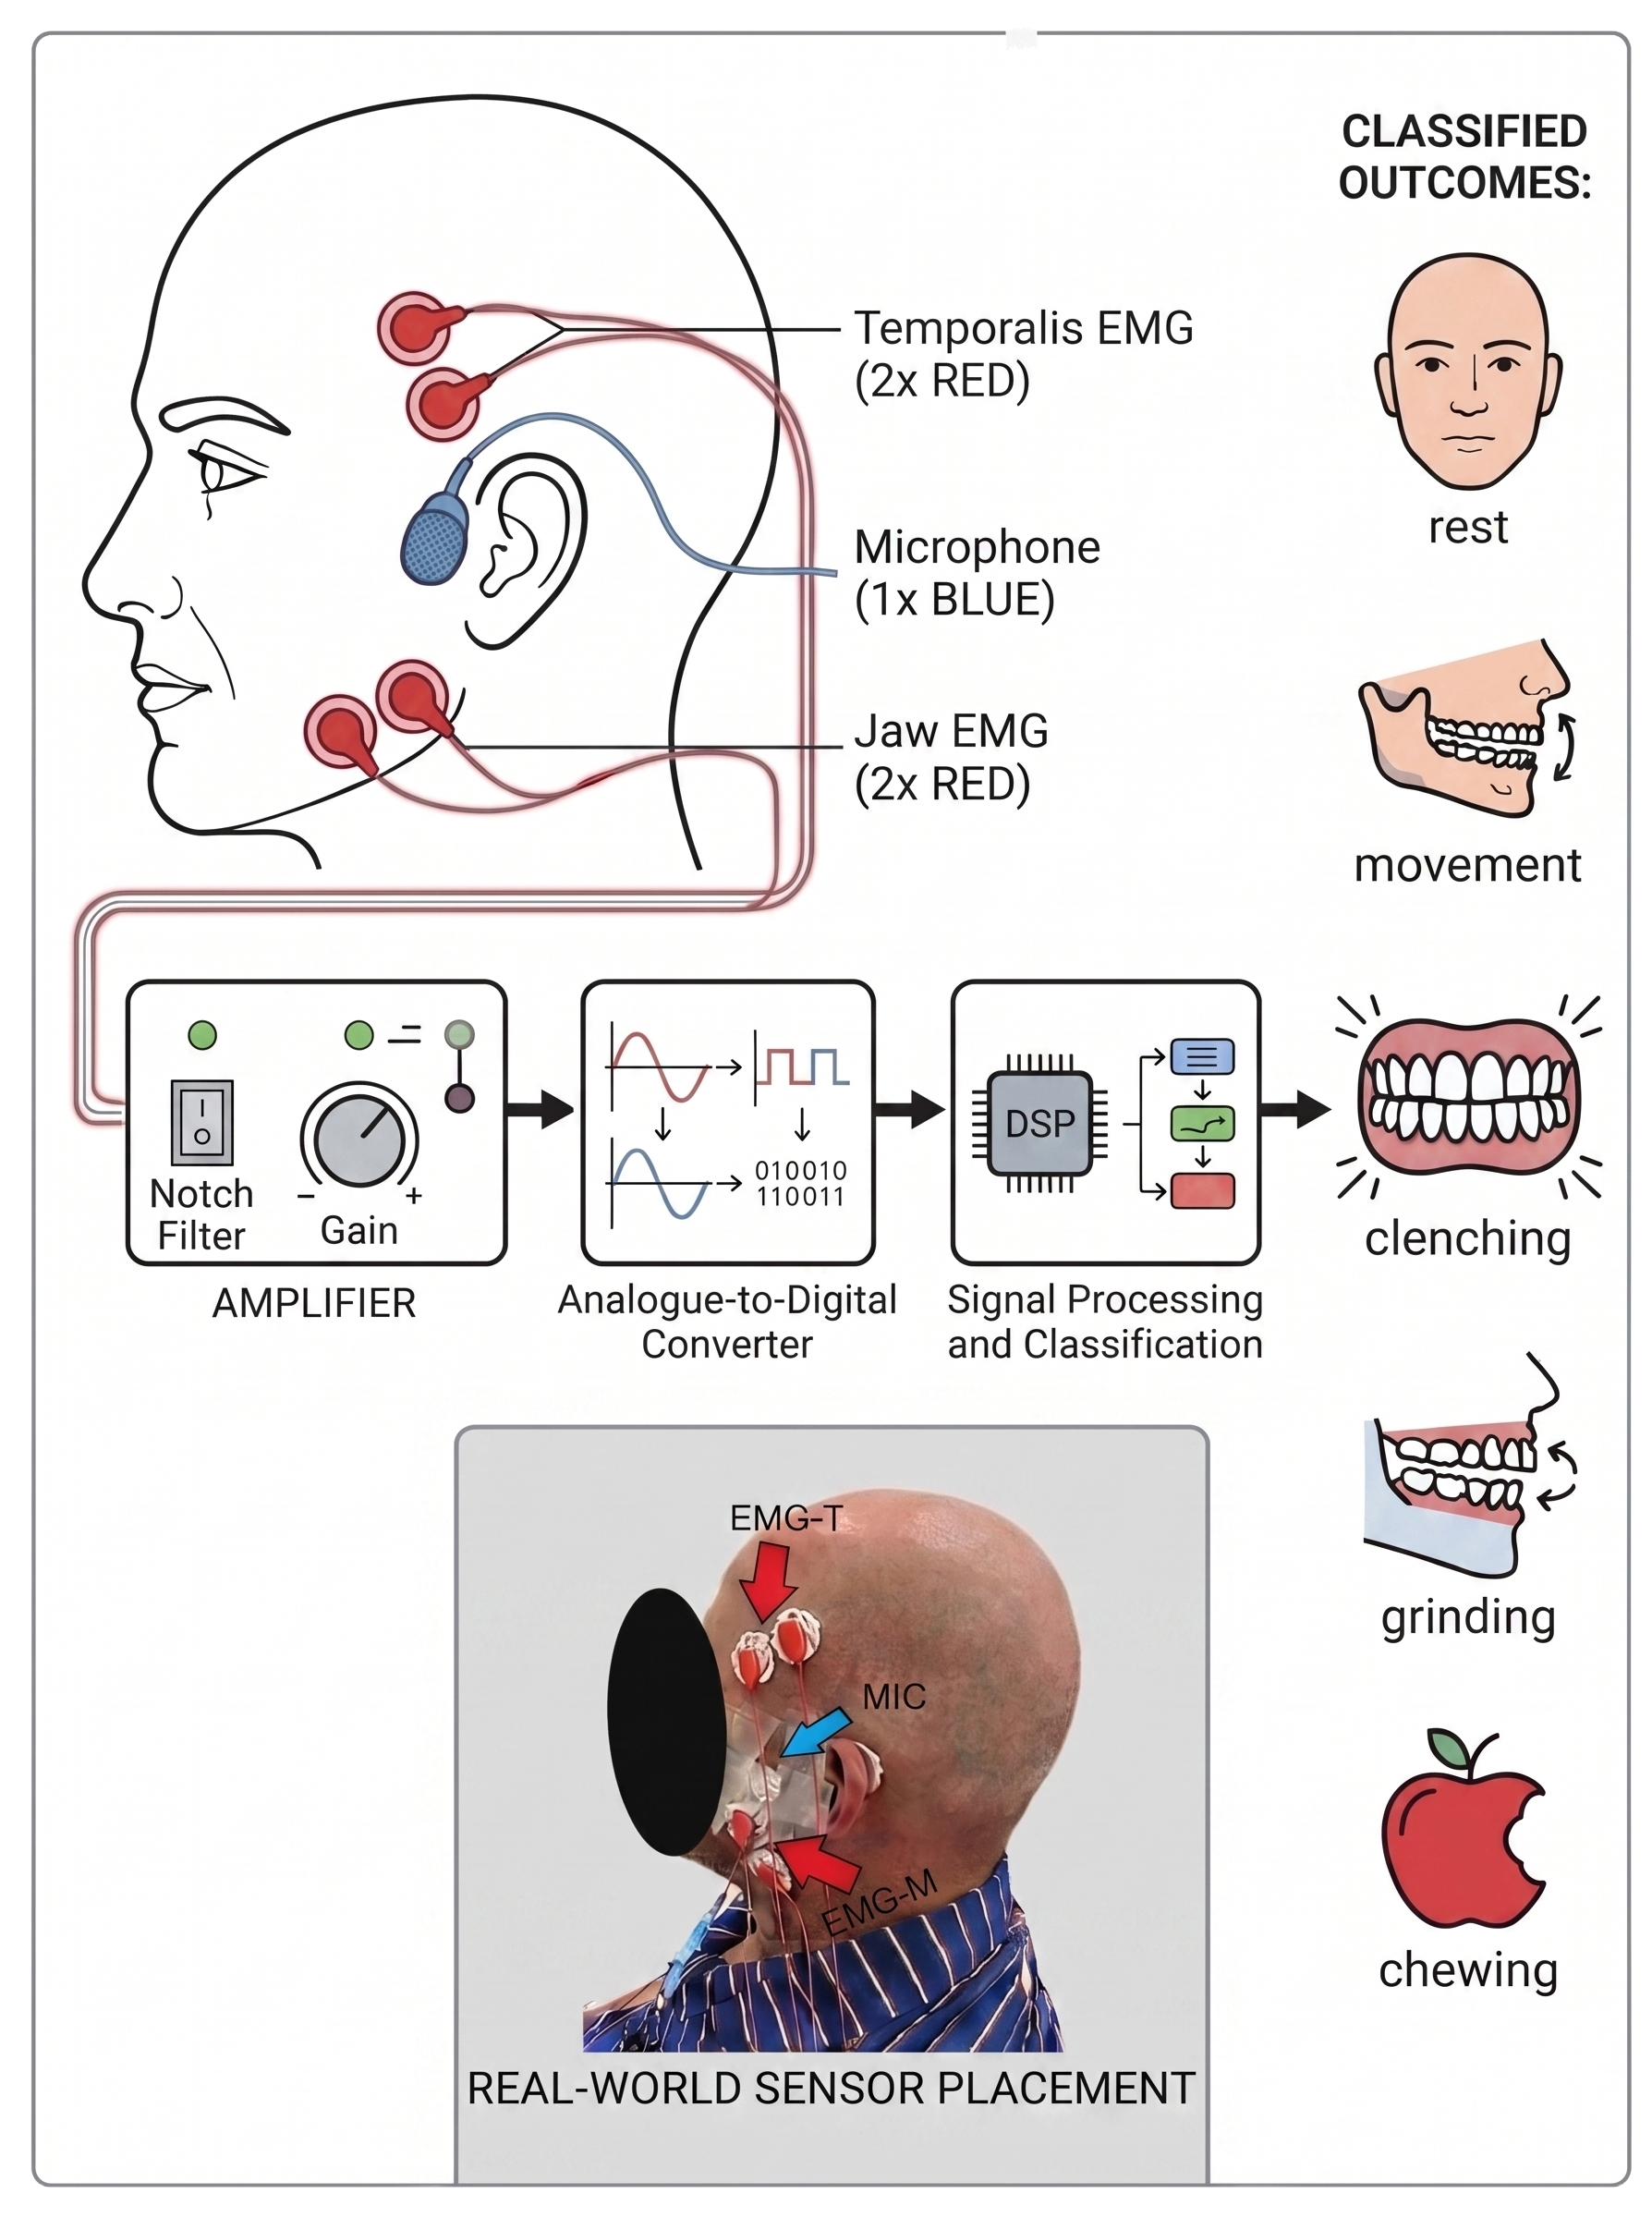
\includegraphics[width=\columnwidth]{Figures/RL4.png}
  \caption{Sensor placement: bipolar surface-EMG pairs over the temporalis (EMG-T) and masseter (EMG-M), with a microphone (MIC) near the temporomandibular joint used only to assist offline review.}
  \label{fig:setup}
\end{figure}

\subsection{Window labelling and the analysable sample}
\label{sec:windows}

Every analysed window lies wholly inside one trigger-marked task interval, so no window spans two conditions or a trigger transition. Windows are cut from the continuously filtered recording and never filtered individually, which would inject an edge transient into each window.

Three exclusions are applied before windowing, each measured rather than assumed (Table~\ref{tab:dataset}). A transition guard of 0.25~s is removed on each side of every trigger edge: over 432 task onsets, muscle activity preceded the marker at 79.9\%, and among the remainder the median lag was 0.054~s and the largest 0.352~s. A startup guard of 0.5~s is removed at the beginning of every recording, because amplifier settling transients appeared in 66 of 100 recordings and all settled within 0.40~s. Quiet-rest windows are drawn only from the five dedicated rest recordings, because trigger-off intervals inside active recordings are unlabelled rather than verified as quiet; the rest class therefore represents quiet laboratory rest, not everyday non-event behaviour.

The recordings were consolidated into five classes: rest, the dedicated quiet-baseline recordings; movement, opening and closing, lateral deviation, protrusion and retrusion; clenching, molar and incisor clench and unilateral bite; grinding; and chewing of cheese, carrots or popcorn, and gum. Bracing and thrusting without tooth contact were not elicited. Chewing was included as a common functional activity and a plausible confound for an ambulatory classifier; because it may also be comparatively easy to recognise, the five-class results are accompanied by a sensitivity analysis that excludes it and by one that collapses the labels into clenching or grinding versus the rest.

Under these rules, 100 recordings yielded 6,173 analysable 1.0-second windows from 99 recordings (Table~\ref{tab:dataset}). Class sizes are strongly unequal: chewing supplies 58.9\%, and within a class the counts differ between participants because they marked the trigger differently (Section~\ref{sec:constraints}). The windows are not independent observations: adjacent windows overlap by 50\%, many come from the same recording, and all come from five people. The participant, not the window, is therefore the unit for generalisation, and all primary metrics are computed within a participant before being summarised~\cite{saeb2017need,little2017using,roberts2017cross}.

\begin{table}[t]
  \caption{Dataset, guards and preprocessing under the trigger-constrained labelling policy.}
  \label{tab:dataset}
  \centering
  \footnotesize
  \begin{tabular*}{\columnwidth}{@{\extracolsep{\fill}}ll@{}}
    \toprule
    Property & Value \\
    \midrule
    Participants / recordings & 5 / 100 (99) \\
    EMG channels analysed & 4 (2 bilateral pairs) \\
    Sampling rate / units & 1200 Hz / arbitrary ADC \\
    Window / stride & 1200 (1.0 s) / 600 (0.5 s) \\
    Transition guard, per edge & 0.25 s \\
    Startup guard, per recording & 0.5 s \\
    \midrule
    Rest windows (5 dedicated recs.) & 590 \\
    Movement windows & 333 \\
    Clenching windows & 799 \\
    Grinding windows & 816 \\
    Chewing windows & 3,635 \\
    \textbf{Total analysed windows} & \textbf{6{,}173} \\
    \midrule
    Mains notches (8 Hz wide) & 60--420 Hz, 7 harm. \\
    Band-pass (Butterworth, order 4) & 20--450 Hz \\
    Filtering mode & Zero-phase, whole rec. \\
    Wavelet / bands & db4, 4 lev.\ / $A_4$, $D_3$, $D_1$ \\
    \bottomrule
  \end{tabular*}
\end{table}

\subsection{Signal validation and the filter chain}
\label{sec:filter}

This stage checks that the recordings contain what the analysis assumes; its effect on classification is RQ1 (Section~\ref{sec:rq1}). The acquisition software applied its own fixed notch, recorded in every metadata sidecar, which removed the 60-Hz fundamental before the data reached disk. Interference survived at the harmonics, 180, 300 and 420~Hz, instead: across all 100 recordings, 62 had more than 30\% of their raw in-band EMG power within $\pm 3$~Hz of a mains multiple, and in the five quiet-rest recordings that share was 91.3--99.8\%.

The chain used in earlier analyses of this dataset, a single 60-Hz notch ($Q=30$) followed by a 20--450-Hz band-pass, removed the only mains frequency that was already absent and passed every frequency that was present: the mains share of in-band power after filtering was 91.4--99.8\%, essentially unchanged (Fig.~\ref{fig:filter_fix}a, c). A filter-response plot of that chain looks entirely conventional, which is why the problem stayed invisible until the response was drawn over the measured spectrum of the data.

The corrected chain notches every mains multiple inside the pass band, from 60 to 420~Hz in steps of 60~Hz, before the same fourth-order Butterworth band-pass from 20 to 450~Hz, a band consistent with direct measurements of jaw and facial EMG~\cite{vanboxtel2001optimal,deluca2010filtering}. Each notch is constant-width, 8~Hz at $-3$~dB, rather than constant-$Q$: at an identical 13\% band cost the constant-width bank left eight times less residual interference. After correction the mains share in the quiet-rest recordings fell to 0.46--0.66\% (Fig.~\ref{fig:filter_fix}b, c). The chain was selected on this interference criterion, which can be specified in advance, and not on held-out score; the distinction is not decorative, because the constant-$Q$ bank scored marginally higher in screening classification, at 0.689 against 0.679 macro-F1, while leaving eight times the interference. All filtering is zero-phase and applied to the whole continuous recording before any window is cut; it suits offline analysis and cannot support a streaming claim.

\begin{figure*}[t]
  \centering
  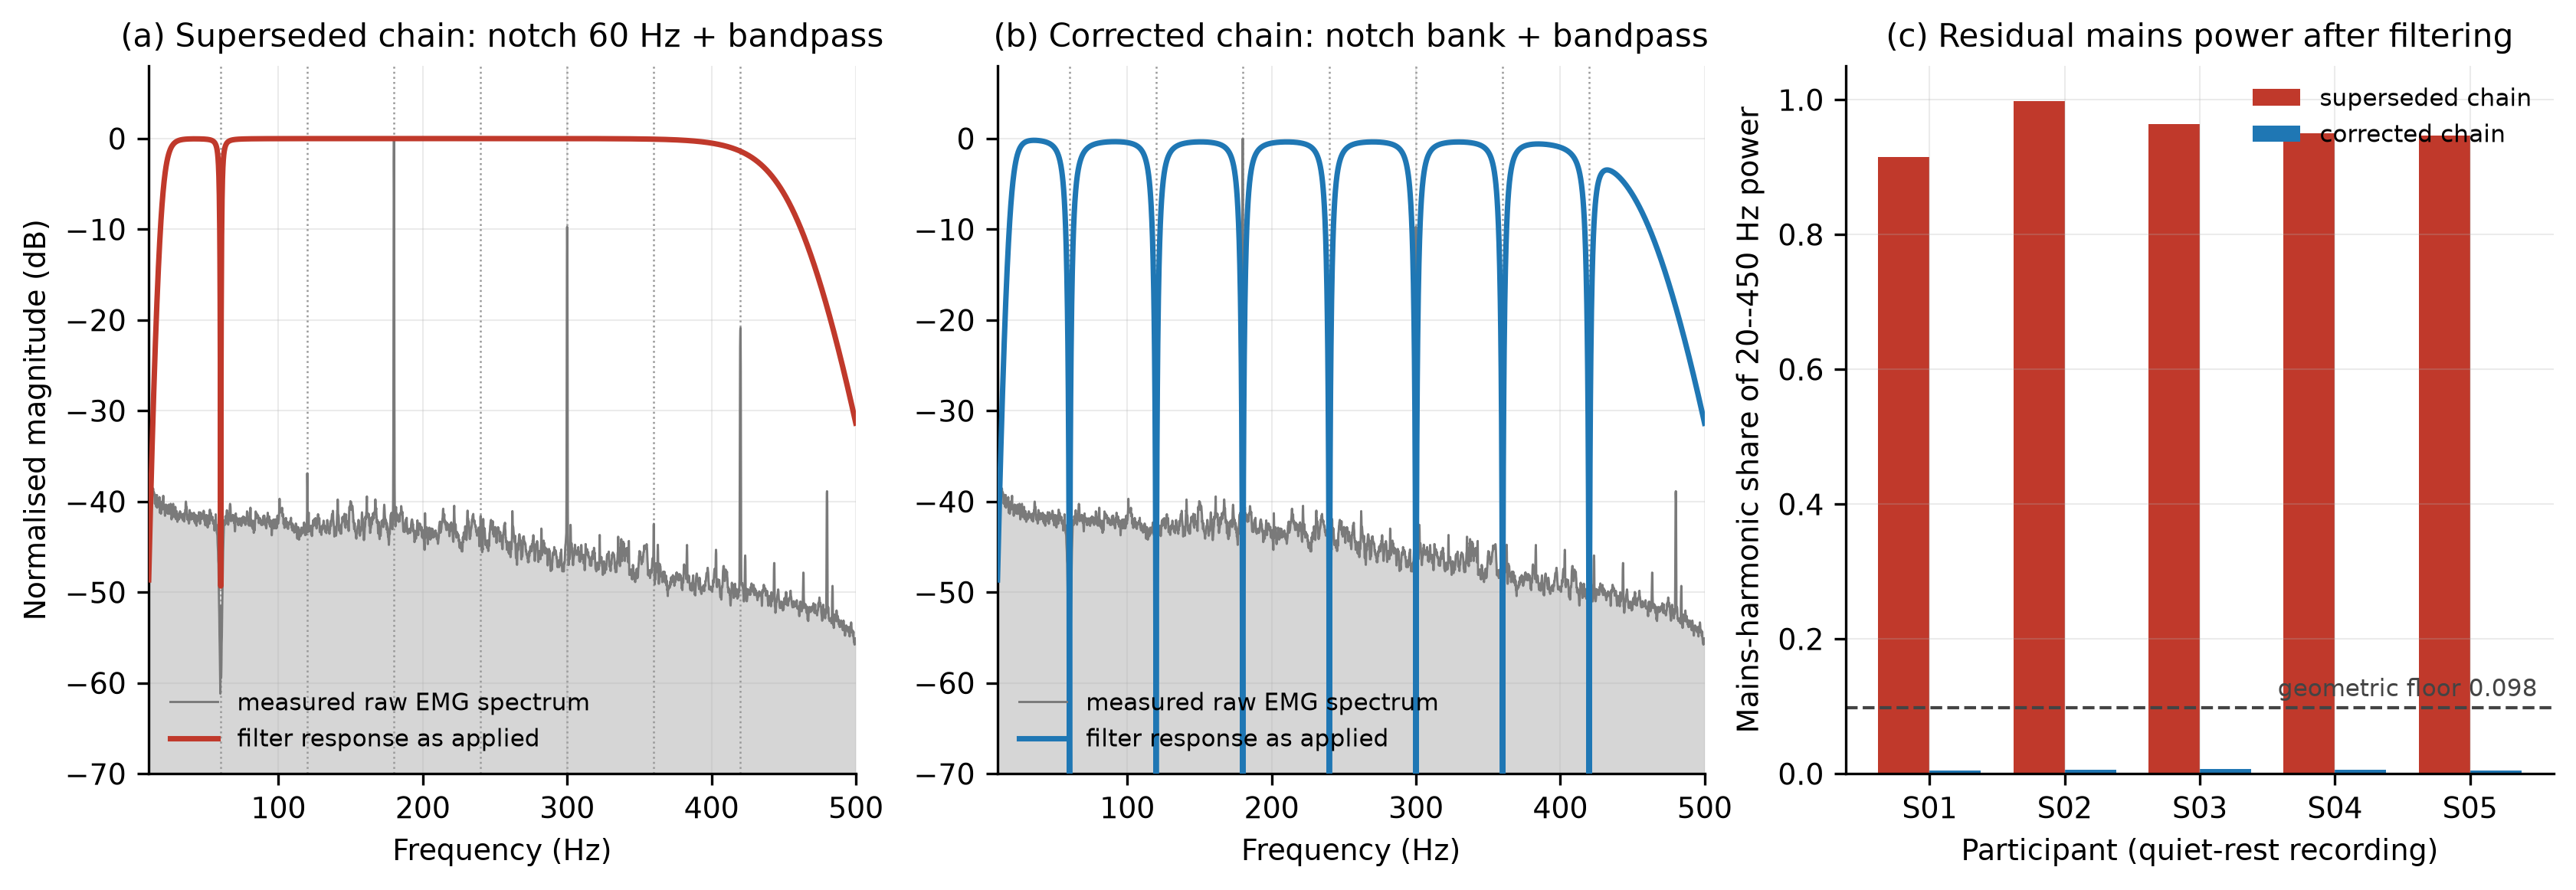
\includegraphics[width=0.72\linewidth]{Figures/filter_defect_and_correction.png}
  \caption{The mains-harmonic defect and its correction. (a) The superseded chain: the 60-Hz notch lands where the hardware had already removed the fundamental, while the harmonic peaks at 180, 300 and 420~Hz pass untouched. (b) The corrected chain: seven constant-width notches land on the peaks. Gray traces are the mean raw spectrum of the five quiet-rest recordings, colored traces the response as applied, dotted lines the mains multiples. (c) Share of 20--450-Hz power within $\pm3$~Hz of a mains multiple, per participant, after each chain; the dashed line marks the 0.098 a white signal would score.}
  \label{fig:filter_fix}
\end{figure*}

\subsection{Normalisation, wavelet decomposition and model}

EMG signals were z-scored per channel using means and standard deviations computed only from the training participants of the fold in question; the list of participants behind each fold's statistics is stored with the fold and asserted not to contain the held-out participant. A per-participant, or transductive, scope is implemented and priced in Section~\ref{sec:constraints}, but no confirmatory number uses it: the strict scope is the one that would support a deployment claim without a fitting session~\cite{besomi2020consensus}.

Figure~\ref{fig:preprocessing} shows the chain on a real excerpt. Signals were then decomposed with the Daubechies-4 wavelet at four levels~\cite{daubechies1992ten,englehart2003robust}, and the sub-branches used $A_4$ (below 38~Hz), $D_3$ (75--150~Hz) and $D_1$ (300--600~Hz, of which only 300--450~Hz survives the band-pass). The pipeline rejects any band its own filter chain has removed unless the configuration declares the exception.

The reference model is a single-branch wavelet convolutional network (Fig.~\ref{fig:architecture}) with one CNN sub-branch per retained band: two 3-tap convolutional blocks of 8 and 16 channels with batch normalisation and a rectified linear unit, averaged over the window's time axis to 16 features per band. The 48 features pass to a multilayer perceptron (MLP) of dimensions $48\rightarrow48\rightarrow32$ with dropout of 0.5, and a final linear layer produces logits for the five classes. The model has 5,901 trainable parameters, or 23.1~KiB at 32-bit precision; Section~\ref{sec:deep_baselines} evaluates an extended member of the same family alongside it.

\begin{figure*}[t]
  \centering
  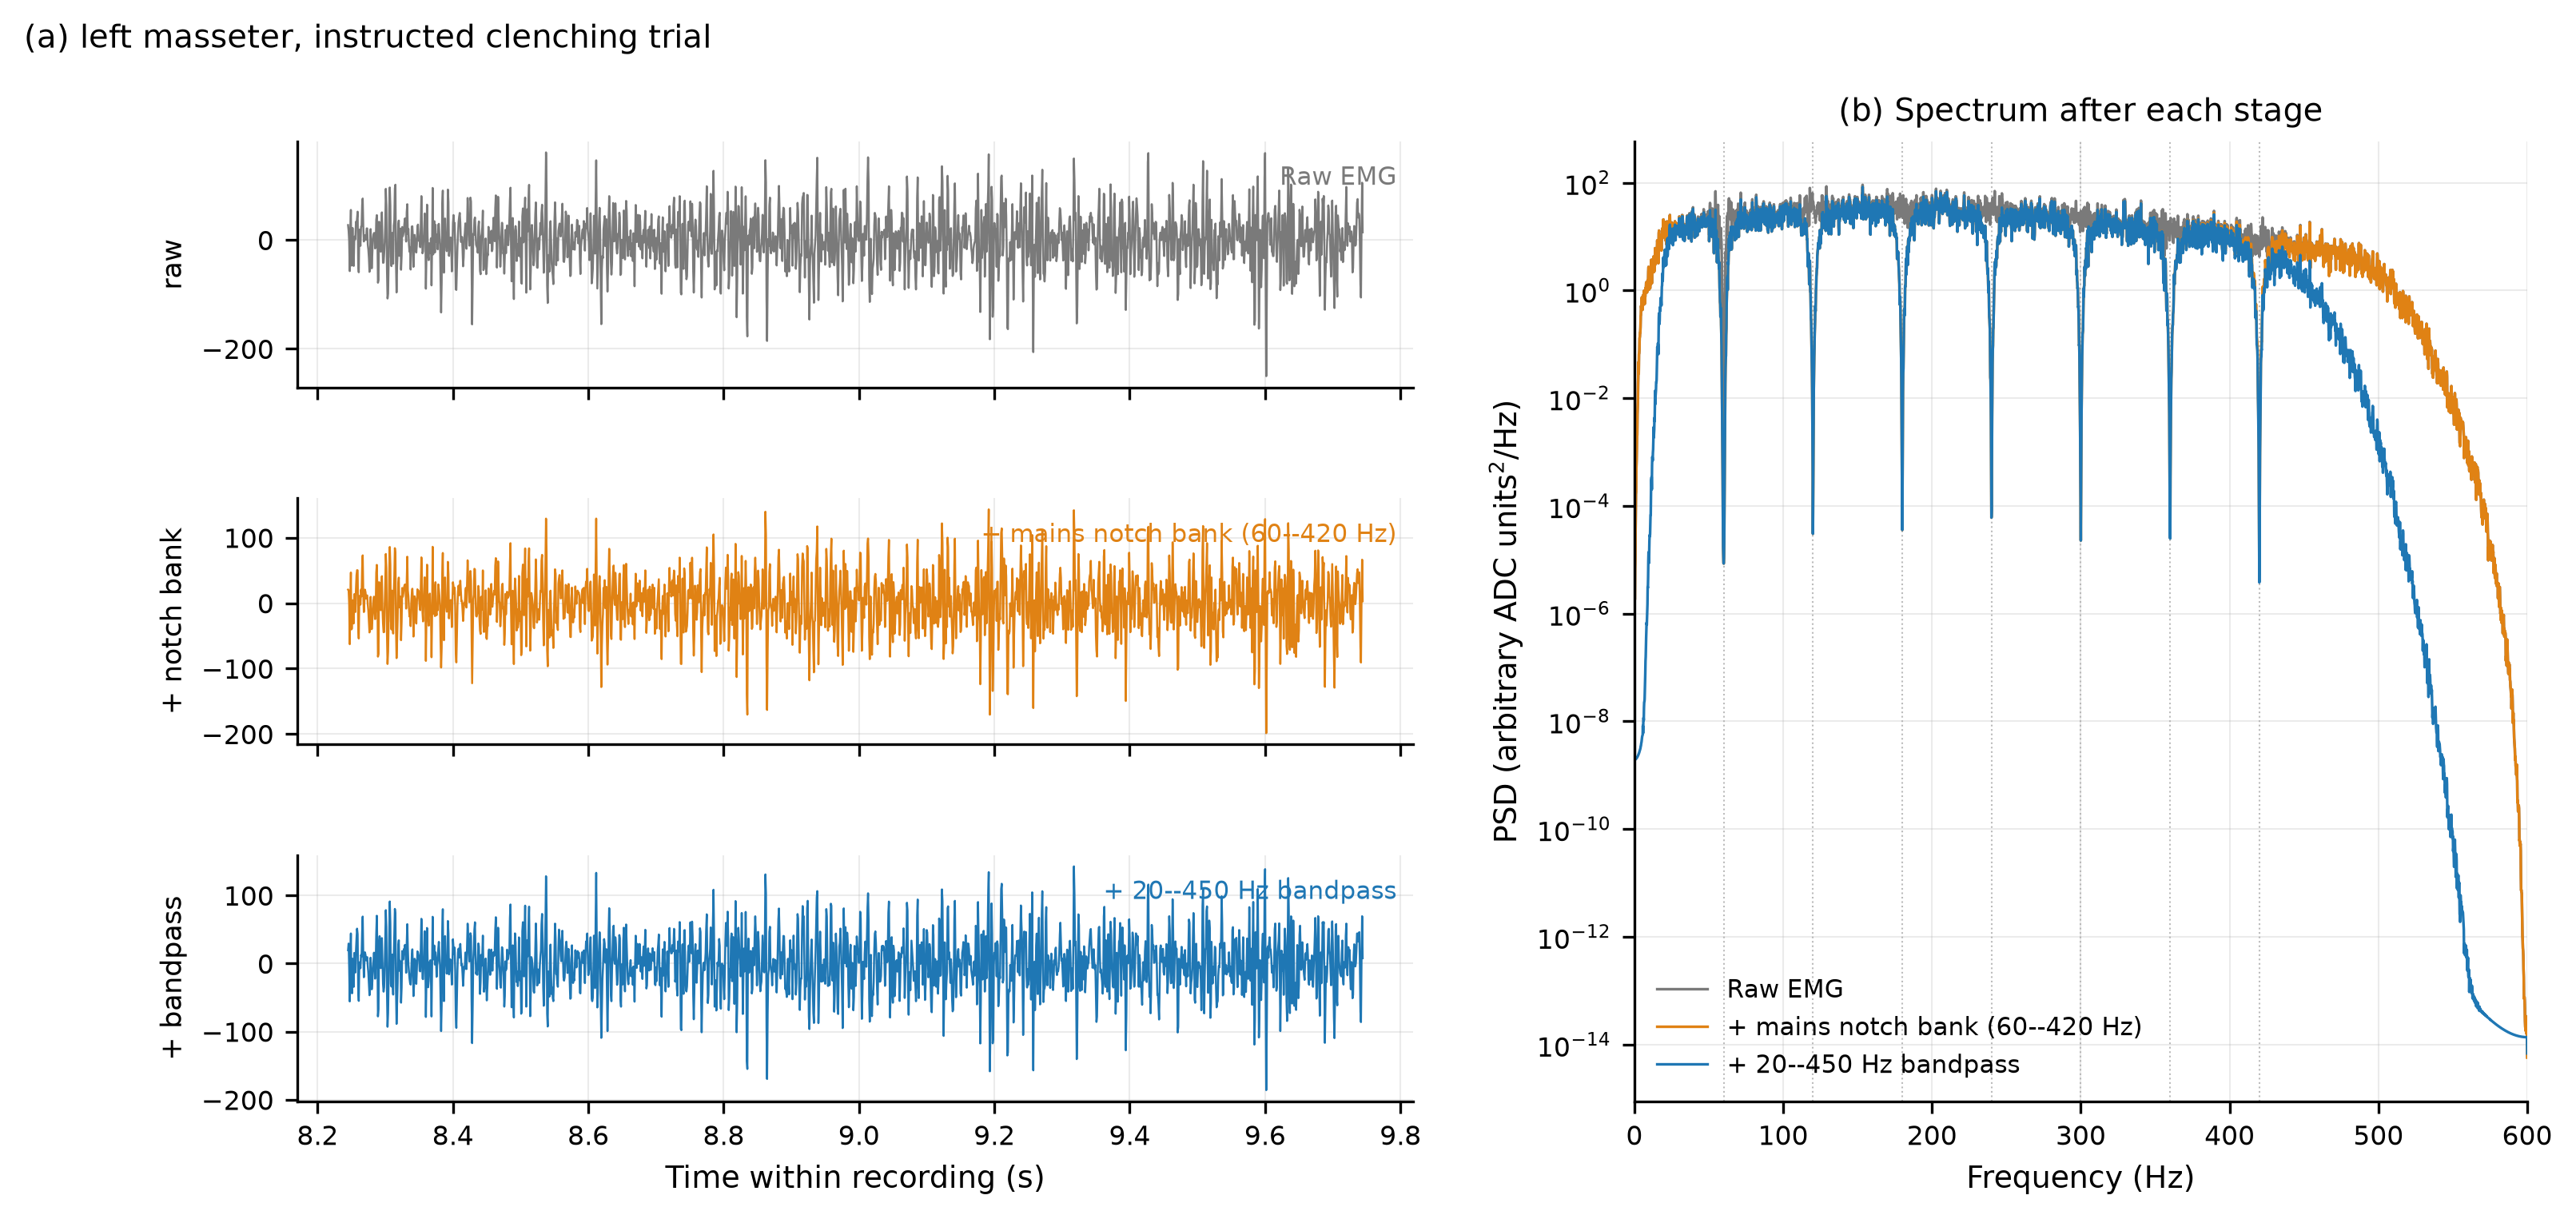
\includegraphics[width=0.6\linewidth]{Figures/preprocessing_stages_5class.png}
  \caption{Production preprocessing on a real excerpt of an instructed clenching trial (left masseter channel). (a) Time domain and (b) power spectrum after each stage: the notch bank removes the seven mains multiples marked by dotted lines, and the band-pass then removes content outside 20--450~Hz. The chain is applied to the continuous recording; windows are cut afterwards.}
  \label{fig:preprocessing}
\end{figure*}

\begin{figure*}[t]
  \centering
  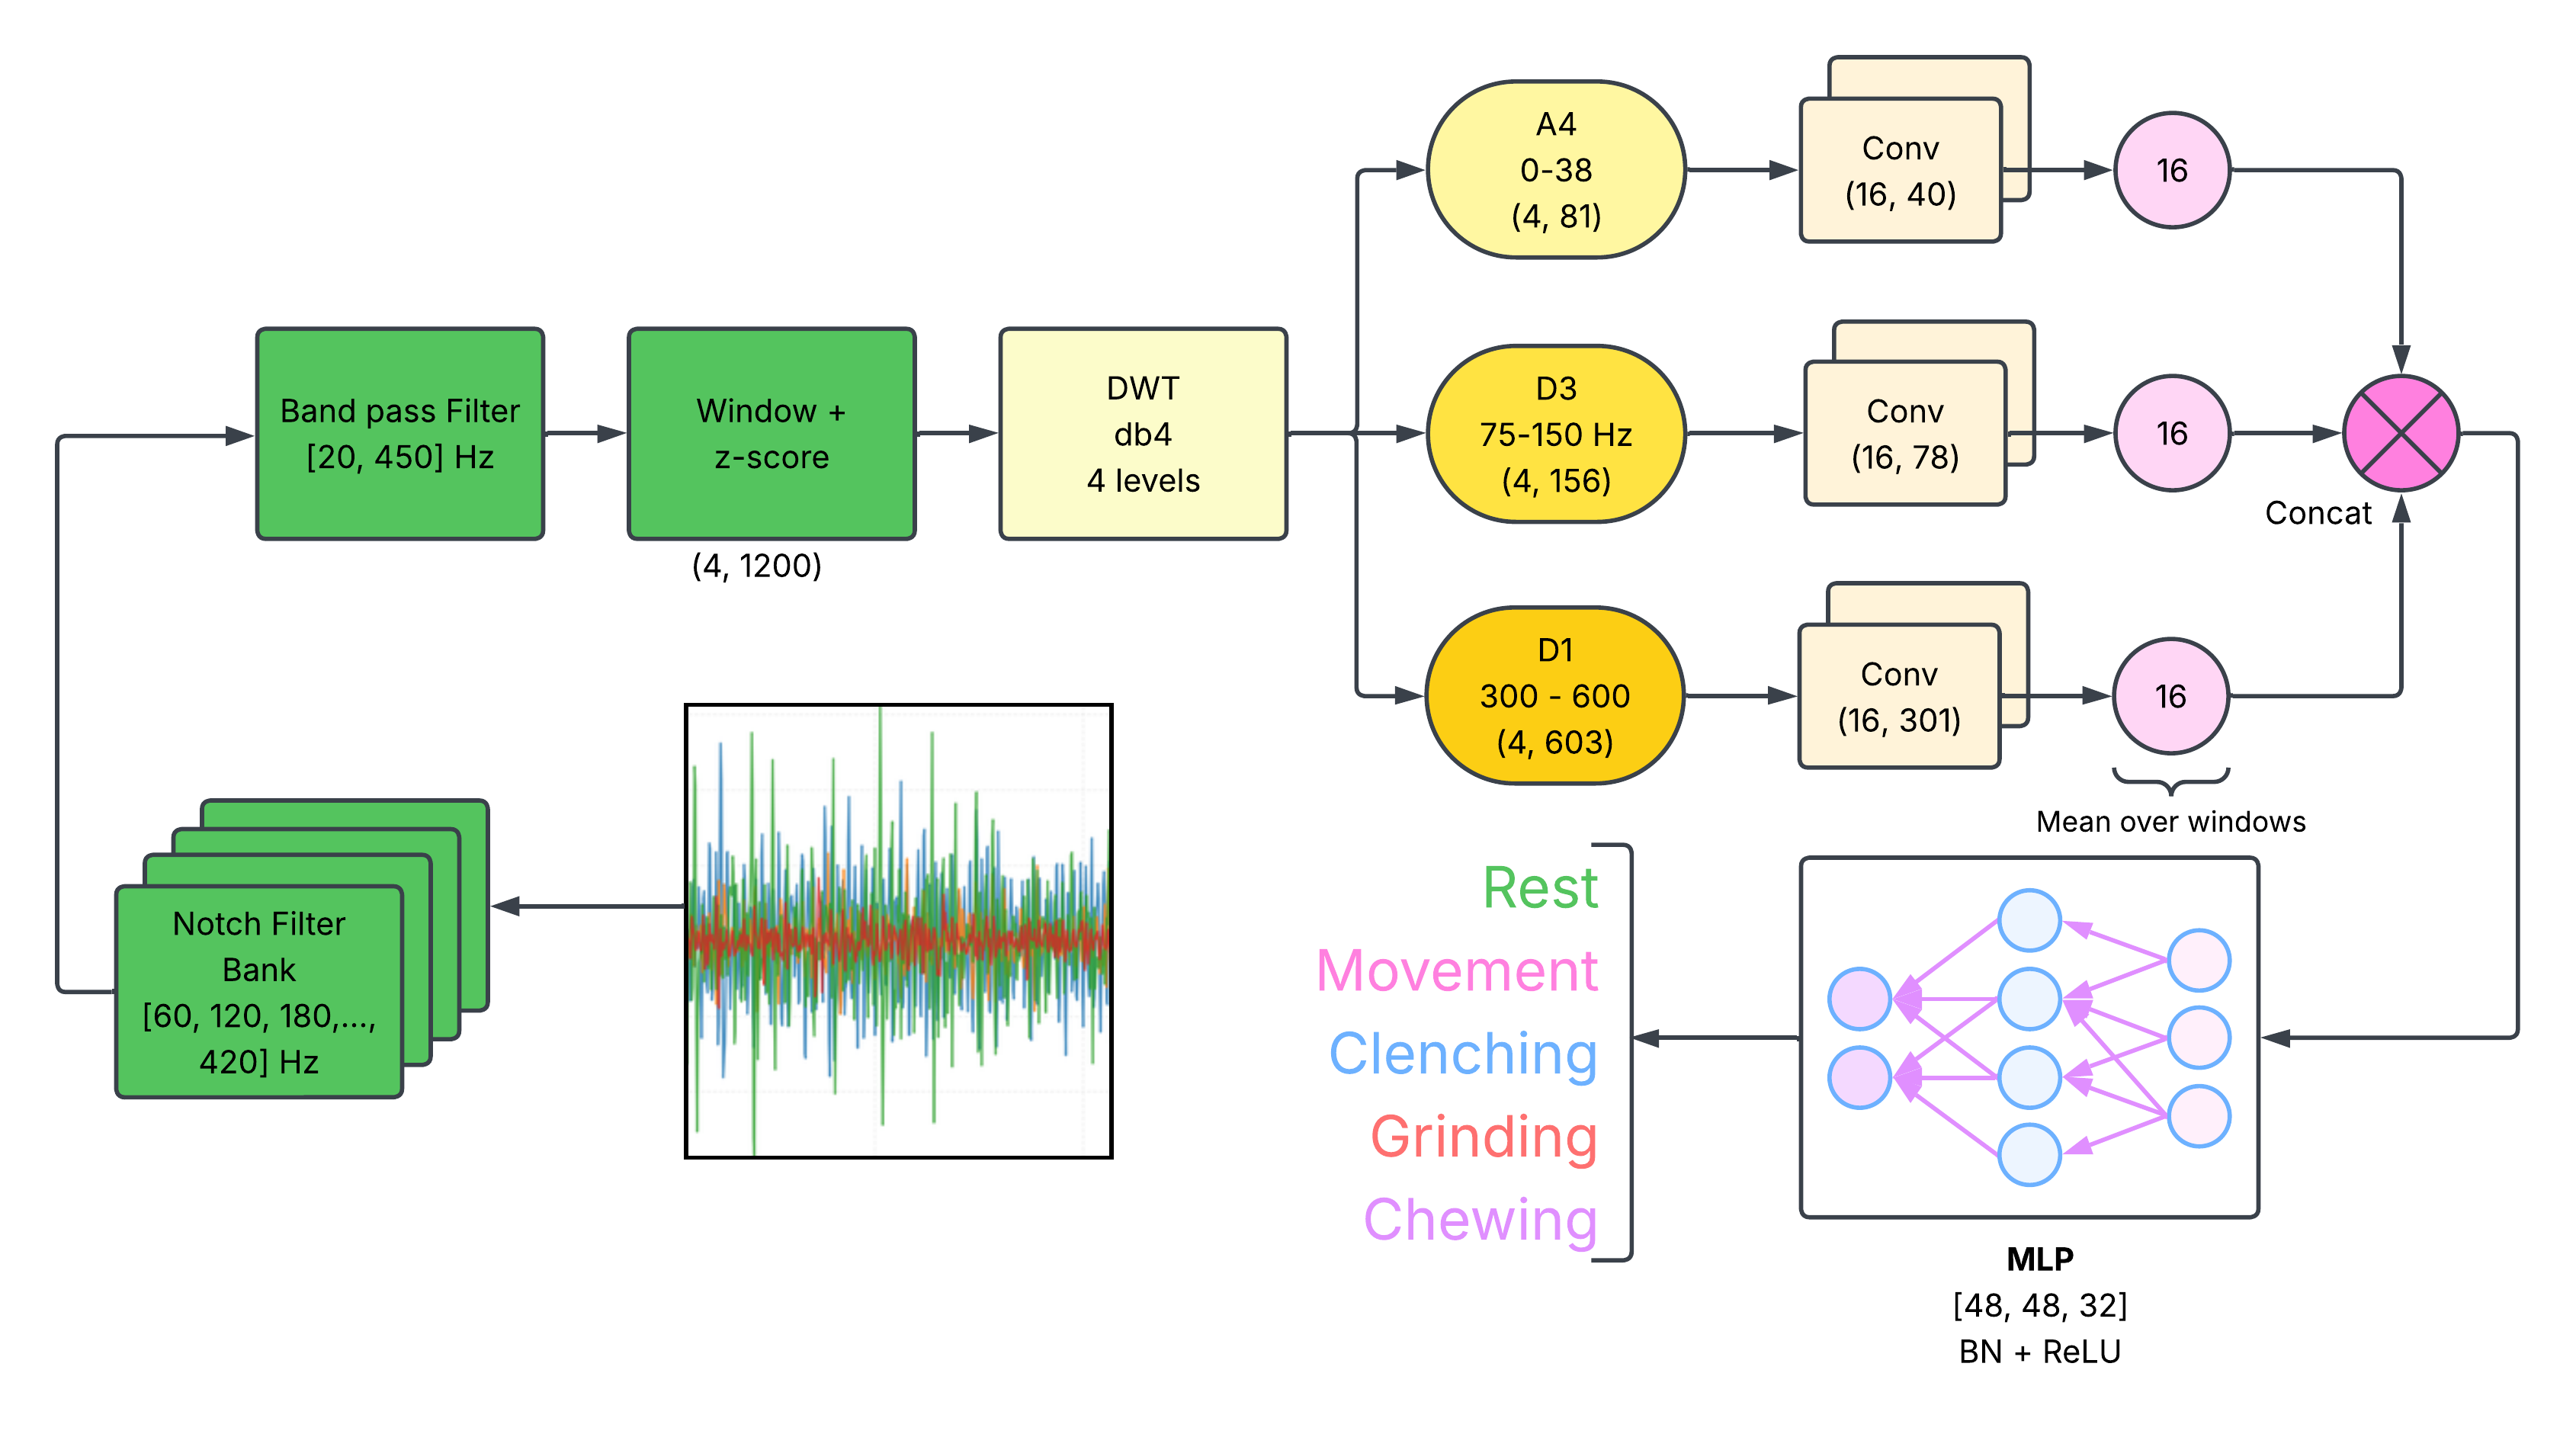
\includegraphics[width=0.64\linewidth]{Figures/Pipeline_V2.png}
  \caption{Signal-to-decision chain of the reference model. The four EMG channels pass through the notch bank and band-pass, are cut into 1.0-s windows, z-scored with training-participant statistics and decomposed with a four-level db4 wavelet transform. The three retained bands, $A_4$ (0--38~Hz), $D_3$ (75--150~Hz) and $D_1$ (300--600~Hz), each pass through two convolutional blocks and are averaged over the window's time axis to 16 features per band; the 48 features enter an MLP of dimensions $48\rightarrow48\rightarrow32$ that produces logits for the five classes. The time-averaging step is the one the extended model of Table~\ref{tab:architectures} removes.}
  \label{fig:architecture}
\end{figure*}

\subsection{Training and evaluation}
\label{sec:training}

Class imbalance was addressed with inverse-frequency class weights recomputed within each outer training fold, and with augmentation of minority-class training windows by amplitude scaling, additive noise and circular shifts, confined structurally to the training partition. Optimisation used AdamW~\cite{loshchilov2019decoupled} and focal loss~\cite{lin2017focal} in PyTorch~\cite{paszke2019pytorch}, with the settings in Table~\ref{tab:hyperparameters}; the loss and learning rate were fixed rather than searched, so that no condition could win by drawing a better hyperparameter.

Evaluation used nested LOSO, because selecting a model and reporting its score on the same held-out data biases the estimate upward~\cite{cawley2010overfitting,varma2006bias}. In each of five outer folds one participant was sealed as the test set and the remaining four entered a participant-grouped inner LOSO loop; every normalisation statistic, class weight and augmentation set was fitted on inner-training participants only. The best epoch was recorded per inner fold by validation macro-F1, and the model was refit on all four outer-training participants for the median of those epochs before the held-out participant was evaluated exactly once. Macro-F1 was the selection objective because accuracy is dominated by chewing~\cite{chicco2020advantages}. Three seeds completed all five outer folds; metrics are computed per seed and then summarised, and no seed is selected as best.

\textbf{Participant-level metrics are primary.} Accuracy, balanced accuracy, macro precision, recall, F1 and one-vs-rest ROC--AUC are computed within each held-out participant and then summarised across the five; pooled-window metrics are descriptive only, because windows within a participant are correlated. No window-level bootstrap intervals or $p$-values are reported: the windows are clustered and overlapping, and with five participants such tests would overstate precision without supporting a population-level claim~\cite{lehmann2006testing,demsar2006statistical}. Held-out probabilities are uncalibrated (expected calibration error 0.063) and must not be read as probabilities~\cite{guo2017calibration}; every AUC, being rank-based, is unaffected.

Two secondary analyses were computed post hoc from the same held-out predictions: chewing windows removed and the remaining four probabilities renormalised, checked against a separately trained four-class model; and predictions collapsed into instructed clenching or grinding versus rest, movement and chewing. Both re-read one model, and the second is task discrimination, not bruxism detection.

\subsection{Feature baselines and the screening harness}
\label{sec:screening}

Two families of measurement come from a deliberately cheap screening harness rather than the confirmatory protocol, and every value it produces is labelled as such. The harness extracts 28 hand-written features per window (for each channel, the log RMS of five db4 bands, the log waveform length and the zero-crossing rate~\cite{phinyomark2012feature}) and fits one model per outer fold with no nested selection, using multinomial logistic regression and histogram gradient boosting~\cite{pedregosa2011scikit}. Because the feature set was chosen after looking at these five participants, screening numbers are directionally reliable and optimistic in level. The harness supplies the before-and-after comparison for RQ1, the hand-engineered baseline for RQ3 and all three measurements for RQ4, on the identical 6,173 windows and five outer folds.

\begin{table}[t]
  \caption{Training and evaluation configuration. The loss and learning rate were fixed rather than searched, so that conditions of the same run differ only in what they were asked to do.}
  \label{tab:hyperparameters}
  \centering
  \footnotesize
  \begin{tabular*}{\columnwidth}{@{\extracolsep{\fill}}ll@{}}
    \toprule
    Hyperparameter & Value \\
    \midrule
    Optimiser & AdamW \\
    Learn.\ rate / weight decay & $10^{-3}$ / $10^{-4}$ \\
    Loss & Focal, $\gamma = 1.5$ \\
    Class weights & Inverse freq., per fold \\
    Dropout / batch size & 0.5 / 64 \\
    Gradient clipping & Norm 1.0 \\
    Epoch budget & Median inner best (15--43) \\
    Seeds & 0, 1, 2 \\
    Outer / inner folds & 5 / 4, ppt-grouped \\
    Normalisation scope & Strict (outer-train ppts) \\
    \bottomrule
  \end{tabular*}
\end{table}

\subsection{Pipeline safeguards}
\label{sec:safeguards}

Three guards run inside the pipeline and refuse to proceed rather than warning: the leakage assertion described above; the band check of Section~\ref{sec:filter}; and a channel-integrity check that computes a rotation-invariant fingerprint of every channel of every recording, groups identical fingerprints, and refuses any run in which a held-out participant's signal also appears in its own training set. The third catches a defect the usual checks cannot: a duplicated channel produces files that are individually well-formed, and the duplication appears only when two files are compared. It costs one pass over the data and is modality-agnostic.

\section{Results}

The confirmatory results come from the EMG conditions of one nested-LOSO run on the corrected signal: five outer folds and three seeds, 6,173 held-out window predictions per seed, 18,519 in total for the five-class task and 7,614 for the separately trained four-class task, every value recomputed from the saved prediction ledgers. Results obtained before the filter correction are superseded and appear only as the contrast arm of RQ1.

\subsection{RQ1: how much of the signal is physiology}
\label{sec:rq1}

The filter chain was changed while the windows, folds and labels were held identical, so the comparison isolates the chain (Table~\ref{tab:filter}, Fig.~\ref{fig:measurement_chain}); the 6,173 windows, their fold assignments and their labels are the same objects in both arms, verified by comparing the two prediction ledgers window by window. Through the superseded chain the confirmatory network reached 55.0\% accuracy, 43.5\% participant-level macro-F1 and a macro one-vs-rest AUC of 0.785; through the corrected chain the matched condition reached 80.9\%, 72.8\% and 0.963, a gain of 29.3 points of macro-F1, and the share of quiet-rest windows misread as clenching or grinding fell from 30.2\% to 6.1\%. The contrast is conservative: the superseded run also searched its loss and learning rate inside each fold, and both arms are the fused condition, so the superseded arm carried an input channel it could exploit. The screening harness reproduces the effect with two much simpler estimators: logistic regression on the 28 band-energy features moved from 37.3\% to 63.9\% macro-F1, and gradient boosting from 38.8\% to 61.3\%. Three estimators of very different capacity move by 22 to 29 points on the same windows, labels and folds.

The per-participant view shows how severe the earlier state was. Through the superseded chain two of the five held-out participants were essentially unclassifiable, P1 at 18.1\% macro-F1 and P2 at 5.4\%, at or below a constant prediction, while P3 to P5 scored 57.6--75.4\%; after the correction the same five span 61.4--82.4\%. What had looked like severe between-participant heterogeneity was substantially an artifact of interference differing between recording sessions.

Three further measurements show that the superseded chain was inert rather than merely suboptimal, and explain the mechanism. First, a control chain with no mains removal at all scored 38.5\% macro-F1 in screening, within 1.2 points of the superseded chain: filtering a fundamental the hardware had already removed was equivalent to not filtering. Second, the interference was the dominant signal. Expressed as each activity's median RMS divided by that participant's own resting RMS, the contrast a classifier must exploit, the superseded chain left chewing at 1.6--7.2$\times$ rest and clenching at 1.6--5.2$\times$; after correction the same quantities are 8.5--35.7$\times$ and 8.1--27.0$\times$ (Fig.~\ref{fig:measurement_chain}c). Third, the superseded chain left a $5.07\times$ spread between the largest and smallest participant median RMS and 20 pairs in which one person's resting EMG exceeded another's active EMG, against $2.97\times$ and none after correction (Fig.~\ref{fig:measurement_chain}d).

\begin{table*}[t]
  \centering
  \caption{RQ1. The EMG filter chain is the only thing that varies: the same 6,173 windows, five outer-fold assignments and labels in every arm, verified window by window across the two prediction ledgers. Residual mains power is the share of 20--450-Hz power within $\pm3$~Hz of a mains multiple, averaged over participant and class cells; a white signal would score 0.098. ``Inv.'' counts participant pairs in which one person's resting EMG exceeded another person's active EMG.}
  \label{tab:filter}
  \footnotesize
  \begin{tabular*}{\textwidth}{@{\extracolsep{\fill}}lcccccc@{}}
    \toprule
    & \multicolumn{3}{c}{Measured signal properties} & \multicolumn{3}{c}{Participant-level macro F1} \\
    \cmidrule(lr){2-4}\cmidrule(lr){5-7}
    EMG chain & \shortstack{Residual\\mains} & \shortstack{Ampl.\\spread} & Inv. & \shortstack{Wavelet\\CNN$^{a}$} & \shortstack{Logistic\\reg.$^{b}$} & \shortstack{Grad.\\boost.$^{b}$} \\
    \midrule
    60 Hz notch only (superseded) & 0.673 & $5.07\times$ & 20 & 43.5\% & 37.3\% & 38.8\% \\
    Band-pass only (control) & 0.671 & $5.02\times$ & 20 & --- & 38.5\% & 39.2\% \\
    \midrule
    \textbf{Mains notch bank, 8 Hz (used)} & \textbf{0.012} & $\mathbf{2.97\times}$ & \textbf{0} & \textbf{72.8\%} & \textbf{63.9\%} & \textbf{61.3\%} \\
    \bottomrule
  \end{tabular*}
  \begin{flushleft}\footnotesize
  $^{a}$Confirmatory nested LOSO, three seeds, five outer folds; both rows the fused condition, the superseded row additionally searching loss and learning rate inside each fold, so the comparison favours the superseded arm. The corrected EMG-only condition scores 72.0\%.
  $^{b}$Screening harness on the 28 EMG features, one fit per outer fold, no nested selection; optimistic in level.
  \end{flushleft}
\end{table*}

\begin{figure*}[t]
  \centering
  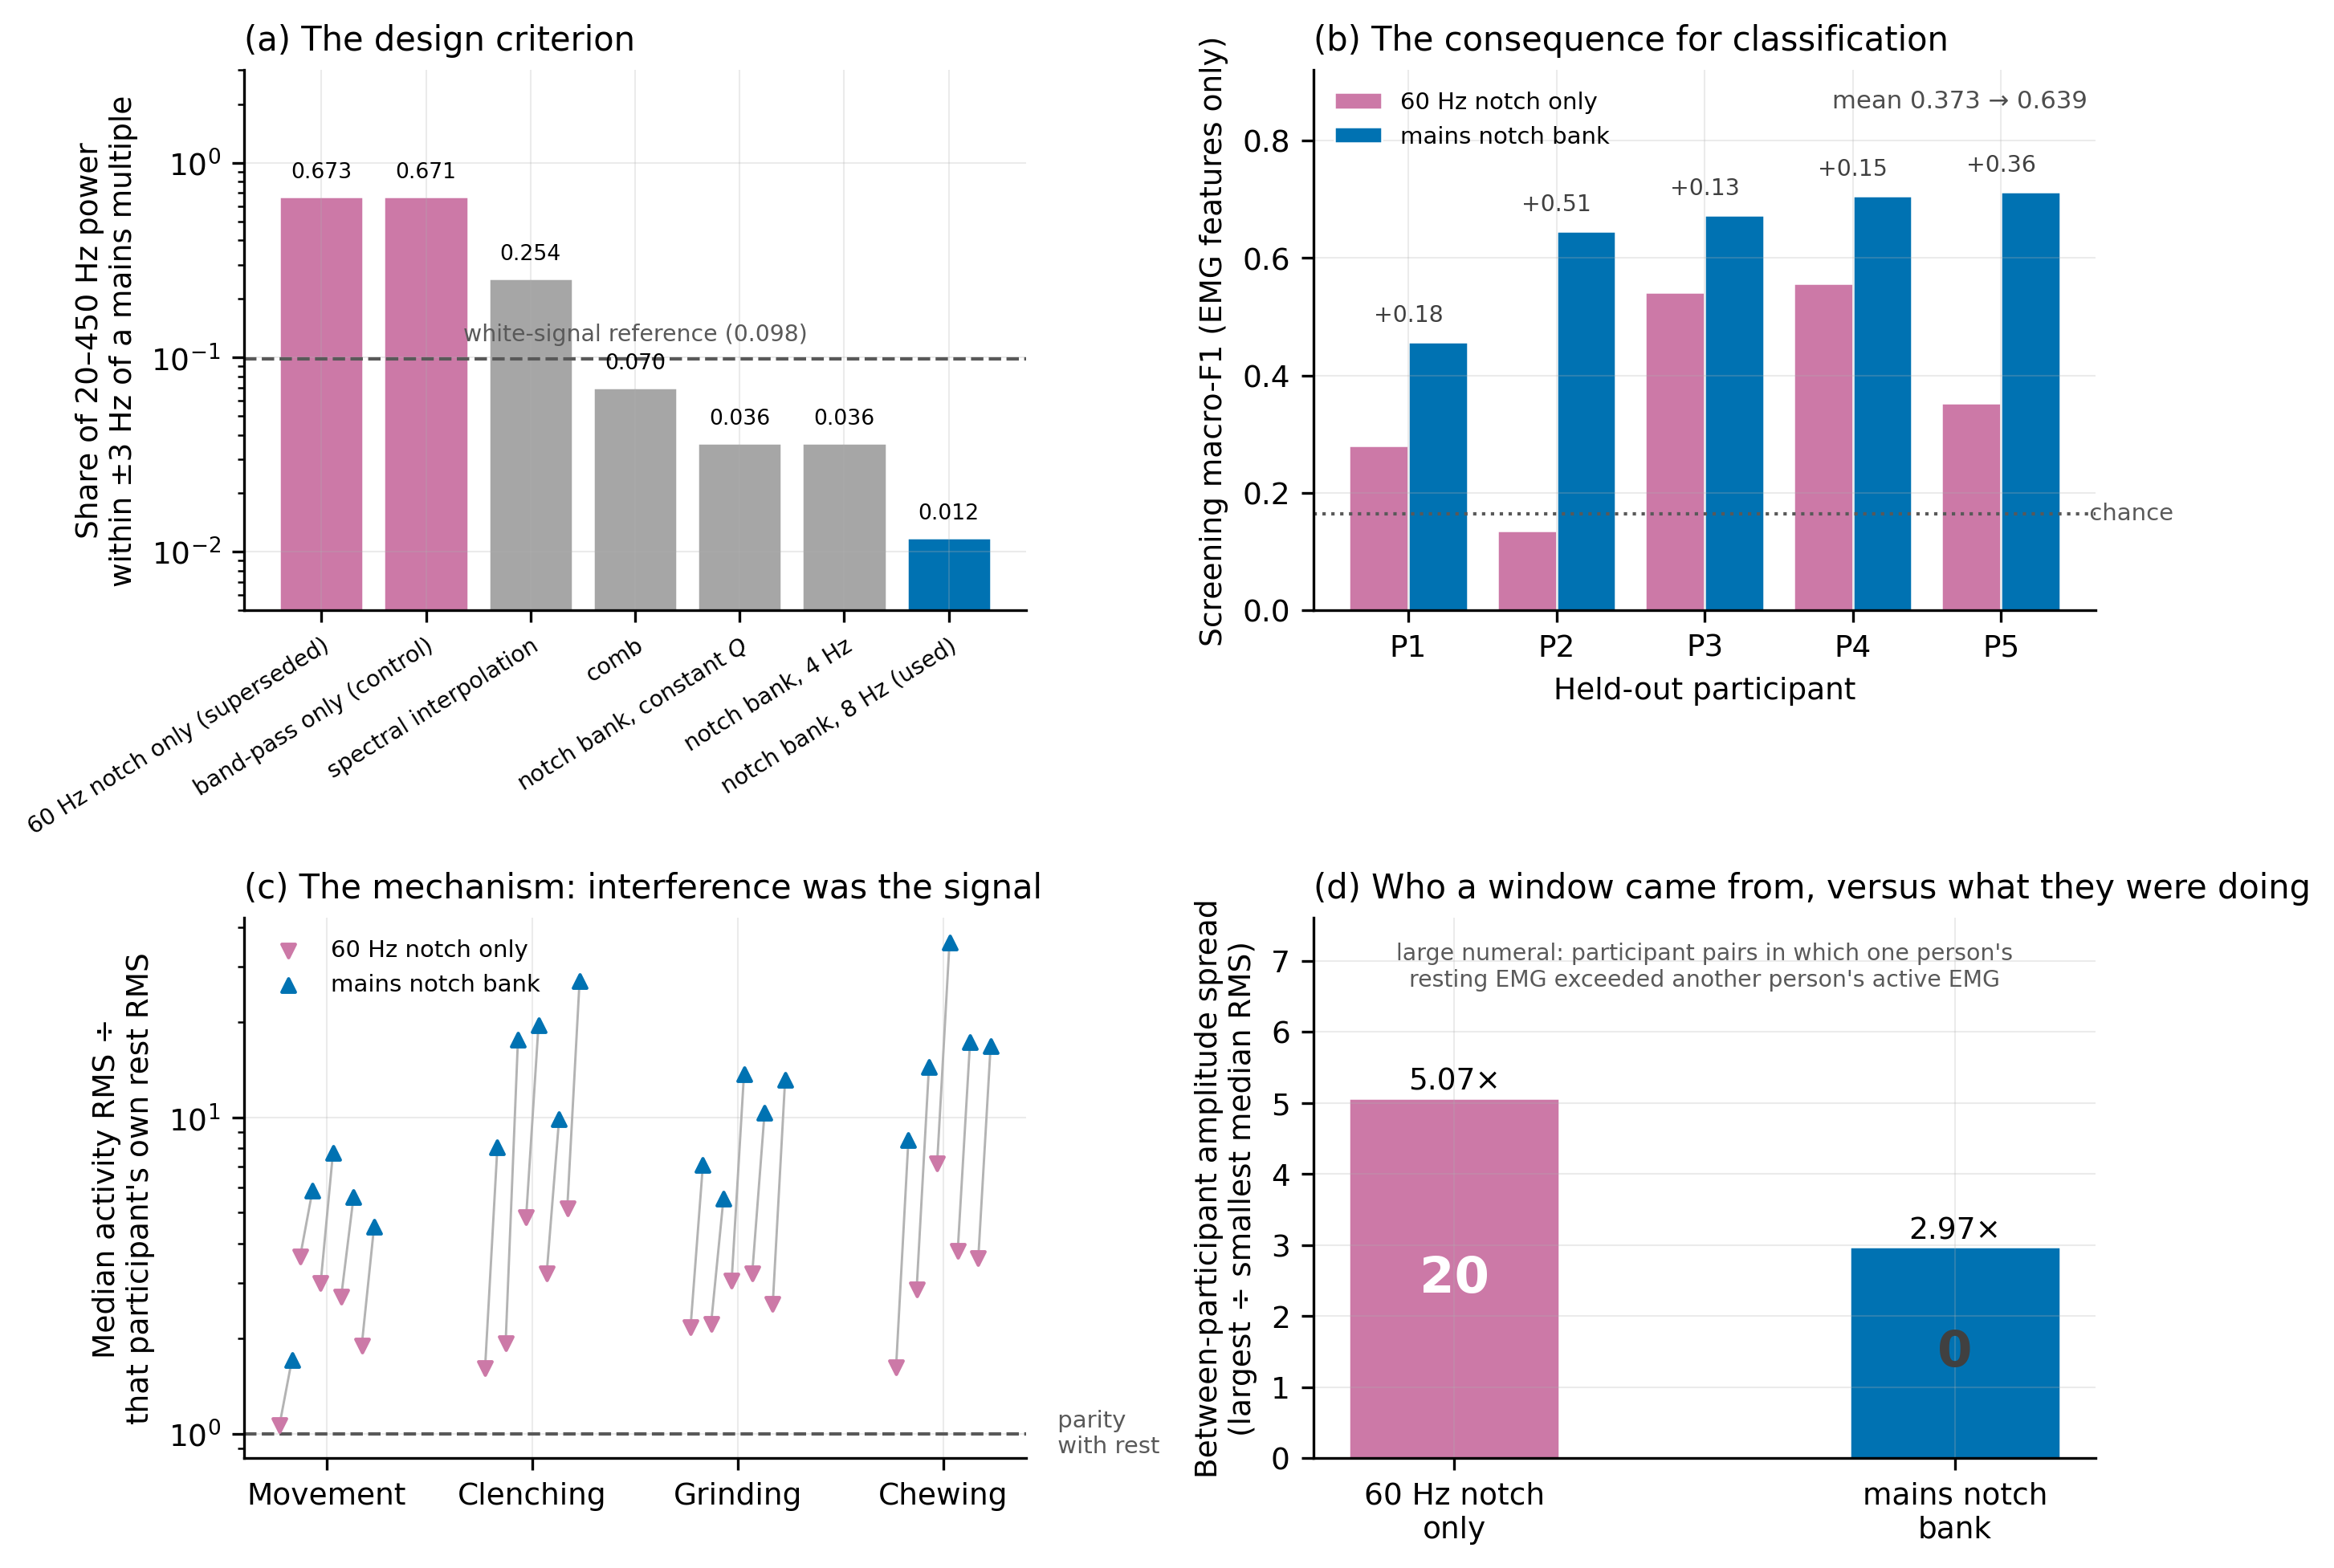
\includegraphics[width=0.62\linewidth]{Figures/v5/measurement_chain.png}
  \caption{The mains-harmonic defect in classification terms. (a) Residual mains power for every candidate chain, against the 0.098 a white signal would score. (b) Screening macro-F1 per held-out participant before and after the correction. (c) Each activity's median RMS divided by that participant's own resting RMS, before (down triangles) and after (up triangles). (d) Between-participant amplitude spread and the number of pairs in which one person's resting EMG exceeded another's active EMG.}
  \label{fig:measurement_chain}
\end{figure*}

\subsection{RQ2: five-class performance on unseen participants}

Averaged over the five held-out participants and three seeds, the model achieved 81.7\% accuracy, 77.6\% balanced accuracy, 72.0\% macro-F1 and a macro one-vs-rest ROC--AUC of 0.958 (Table~\ref{tab:results}). Seed-to-seed variation was small relative to variation between participants, macro-F1 74.5\%, 69.9\% and 71.4\% across seeds; pooling held-out windows across participants, a descriptive summary only, gives 80.7\% accuracy and 71.5\% macro-F1.

Quiet rest reached 77.1\% precision, 91.4\% recall, an F1 of 83.6\% and an AUC of 0.958: the second-best-separated class after chewing and the best-recalled of the five. Per-class ROC curves are shown in Fig.~\ref{fig:roc}, with one caution. Movement reaches an AUC of 0.937, almost identical to clenching's 0.936, yet its precision is 34.4\% against clenching's 70.5\%; AUC is insensitive to class size and precision is not~\cite{saito2015precision,davis2006relationship}, so a reader who looks only at AUC will overestimate how usable the small classes are.

\begin{table*}[t]
  \centering
  \caption{Five-class performance on the corrected signal. Upper block: participant-level means over the five held-out participants and three seeds. Lower block: per-class values on pooled held-out windows, averaged over seeds, with one-vs-rest AUC from held-out probabilities. Values describe this five-participant dataset and are not population-level tests.}
  \label{tab:results}
  \footnotesize
  \begin{tabular*}{\textwidth}{@{\extracolsep{\fill}}lcccccc@{}}
    \toprule
    Method / class & Accuracy & Precision & Recall & F1 & AUC & Windows \\
    \midrule
    \multicolumn{7}{l}{\emph{Participant-level means, five held-out participants $\times$ three seeds}}\\
    \textbf{Wavelet CNN, 4-channel EMG} & \textbf{81.7\%} & \textbf{73.7\%} & \textbf{77.6\%} & \textbf{72.0\%} & \textbf{0.958} & 6,173 \\
    Logistic regression, band energies$^{a}$ & 78.3\% & -- & -- & 63.9\% & 0.965 & 6,173 \\
    Gradient boosting, band energies$^{a}$ & 74.8\% & -- & -- & 61.3\% & 0.914 & 6,173 \\
    \midrule
    \multicolumn{7}{l}{\emph{Wavelet CNN, per class, pooled held-out windows}}\\
    Rest & -- & 77.1\% & 91.4\% & 83.6\% & 0.958 & 590 \\
    Movement & -- & 34.4\% & 69.8\% & 46.0\% & 0.937 & 333 \\
    Clenching & -- & 70.5\% & 66.0\% & 68.1\% & 0.936 & 799 \\
    Grinding & -- & 67.9\% & 69.5\% & 68.6\% & 0.928 & 816 \\
    Chewing & -- & 97.3\% & 85.8\% & 91.1\% & 0.981 & 3,635 \\
    Macro average & 80.7\% & 69.4\% & 76.5\% & 71.5\% & 0.948 & 6,173 \\
    \bottomrule
  \end{tabular*}
  \begin{flushleft}\footnotesize
  $^{a}$Screening harness (Section~\ref{sec:screening}), optimistic in level, which makes the network's margin over these rows conservative; the harness stores no per-class table. Pooled-window macro AUCs: 0.948 CNN, 0.944 logistic regression, 0.894 gradient boosting.
  \end{flushleft}
\end{table*}

\begin{figure}[t]
  \centering
  
\includegraphics[width=0.8\linewidth]{Figures/v5/five_class_roc_curves.png}
  \caption{One-vs-rest ROC curves for the five classes, pooled over the held-out windows of seed 0, chosen by the fixed rule of lowest seed index. Legend values are that seed's; three-seed means are in Table~\ref{tab:results}.}
  \label{fig:roc}
\end{figure}

\subsection{Where the errors are}
\label{sec:diagnostics}

The highest per-class F1 was chewing's at 91.1\%, the lowest movement's at 46.0\%. Movement's is a precision problem: recall 69.8\% and AUC 0.937, but precision 34.4\%, because it is the smallest class at 333 windows and absorbs 9.9\% of the eleven-times-more-numerous chewing windows. Clenching and grinding are the hardest pair to separate, with 19.5\% of clenching windows labelled grinding and 14.5\% of grinding windows clenching, together the majority of both classes' errors. Rest had the highest recall of any class, and its dominant error was into grinding at 7.5\%, against 0.3\% into clenching, so confusion between quiet rest and the clenching-or-grinding group occurred in 7.7\% of rest windows (Fig.~\ref{fig:diagnostics}a), the errors that approximate false alarms under the limited quiet-rest condition.

Table~\ref{tab:persubject} and Fig.~\ref{fig:diagnostics}b report each held-out participant: accuracy from 73.4\% to 90.7\%, macro-F1 from 63.2\% to 80.5\% and macro AUC from 0.904 to 0.981. P4 pairs the lowest accuracy with the second-highest AUC (74.0\%, 0.981), so its windows are ranked well and the loss lies in where the decision boundaries fall; P1 pairs the lowest AUC and macro-F1 with 1,692 of the 6,173 windows, so it dominates any pooled summary while counting as one of five at participant level. With five participants the tabulated standard deviations describe the sample, not a sampling distribution.

t-SNE~\cite{vandermaaten2008visualizing} of the 32-dimensional penultimate representation (Fig.~\ref{fig:tsne}) reproduces both error patterns: chewing occupies several well-separated regions, rest forms tight islands, clenching and grinding interleave, and movement scatters along the borders of the larger classes; t-SNE distances are not metric, so the embedding is corroboration only.

\begin{figure*}[t]
  \centering
  
\includegraphics[width=0.44\linewidth]{Figures/v5/confmatrx_5class.png}
  \hfill
  
\includegraphics[width=0.355\linewidth]{Figures/v5/five_class_per_participant.png}
  \caption{Held-out behaviour of the reference model. (a) Confusion matrix pooled across the five LOSO folds of seed 0, as counts and row-normalised recall. (b) Macro-F1 per held-out participant: bars are the mean over three seeds, open markers the individual seeds, and the label inside each bar that participant's held-out window count.}
  \label{fig:diagnostics}
\end{figure*}

\begin{table}[t]
  \caption{Five-class performance for each held-out participant, averaged over three seeds.}
  \label{tab:persubject}
  \centering
  \footnotesize
  \begin{tabular*}{\columnwidth}{@{\extracolsep{\fill}}lrrrr@{}}
    \toprule
    Held out & $n$ & Acc. & Macro F1 & Macro AUC \\
    \midrule
    Participant 1 & 1,692 & 73.4\% & 63.2\% & 0.904 \\
    Participant 2 & 1,007 & 90.7\% & 72.6\% & 0.957 \\
    Participant 3 & 1,133 & 83.7\% & 71.3\% & 0.967 \\
    Participant 4 & 1,167 & 74.0\% & 72.2\% & 0.981 \\
    Participant 5 & 1,174 & 86.7\% & 80.5\% & 0.980 \\
    \midrule
    Mean & 6,173 & 81.7\% & 72.0\% & 0.958 \\
    SD & --- & 7.7 & 6.1 & 0.032 \\
    \bottomrule
  \end{tabular*}
\end{table}

\begin{figure}[t]
  \centering
  
\includegraphics[width=0.76\linewidth]{Figures/v5/tsne_5class.png}
  \caption{t-SNE of the 32-dimensional penultimate representation for the held-out windows of one seed, coloured by class; each held-out window appears exactly once.}
  \label{fig:tsne}
\end{figure}

\subsection{Secondary analyses with rest}
\label{sec:secondary}

Excluding chewing leaves a four-class problem that yielded 77.7\% accuracy, 75.7\% macro-F1 and a macro AUC of 0.942 at participant level (Table~\ref{tab:sensitivity}). Removing chewing lowers accuracy by 4.0 points but raises macro-F1 by 3.7, because the metric is no longer dominated by one large, easily separated class; a model trained separately on the same four classes reaches 75.8\% macro-F1, confirming that the post-hoc values are not an artifact of renormalisation.

Treating clenching and grinding as the positive group yielded 92.5\% accuracy, 84.8\% sensitivity, 95.3\% specificity and an AUC of 0.970 on pooled windows, and 93.0\% accuracy with a participant-level macro-F1 of 89.3\%. Within the quiet-rest condition, 7.7\% of rest windows (45, 50 and 42 of 590 across the three seeds) fell on the tooth-contact side. At a 0.5-s decision interval that corresponds to roughly 550 false alarms per hour if the background were quiet rest throughout, a quantity this design cannot estimate.

\begin{table*}[t]
  \caption{Secondary analyses computed post hoc from the held-out five-class predictions, averaged over three seeds. These re-read one trained model; they are not separately trained tasks.}
  \label{tab:sensitivity}
  \centering
  \footnotesize
  \begin{tabular*}{\textwidth}{@{\extracolsep{\fill}}lcccccc@{}}
    \toprule
    Analysis & Accuracy & Precision & Recall & Specificity & F1 & AUC \\
    \midrule
    Excluding chewing$^{a}$ & 75.4\% & 74.9\% & 76.1\% & -- & 75.4\% & 0.919 \\
    Collapsed binary$^{b}$ & 92.5\% & 86.4\% & 84.8\% & 95.3\% & 85.5\% & 0.970 \\
    \bottomrule
  \end{tabular*}
  \begin{flushleft}\footnotesize
  Values are pooled over held-out windows; the participant-level means are 77.7\% accuracy, 75.7\% macro-F1 and 0.942 AUC excluding chewing, and 93.0\%, 89.3\% and 0.968 for the collapsed binary analysis.
  $^{a}$Macro values across rest, movement, clenching and grinding after removing chewing windows and renormalising the remaining probabilities.
  $^{b}$Instructed clenching and grinding treated as positive; rest, movement and chewing as the comparison group. Task discrimination, not clinical diagnosis.
  \end{flushleft}
\end{table*}

\subsection{RQ3, part one: the learned representation against hand-engineered features}
\label{sec:rq3}

On the identical windows and folds, the screening harness reached 63.9\% macro-F1 at 78.3\% accuracy with logistic regression on the 28 band-energy features, and 61.3\% at 74.8\% with gradient boosting (Table~\ref{tab:results}). The network's 72.0\% macro-F1 exceeds these by 8.1 and 10.6 points, a conservative margin given the harness's optimism, and stable in direction across two very different estimators.

The AUC column does not follow. Logistic regression reaches a participant-level macro AUC of 0.965 against the network's 0.958, a difference smaller than the network's own seed-to-seed range, so the two models rank held-out windows about equally well and the network's advantage lies in where its decision boundaries fall. That is why macro-F1 rather than AUC was the prespecified selection objective.

One qualification matters more than the margin: the advantage was much smaller before the measurement chain was corrected. Through the superseded chain the network reached 43.5\% macro-F1 against 39.3\% and 40.1\% for the two baselines, a margin of about four points obtained by a network that additionally searched its hyperparameters and carried a microphone branch. The near-parity had been read as evidence that the architecture contributed nothing over band energies; the reading was correct about the numbers and wrong about the cause: when the dominant variance in a window is interference amplitude, a per-band pooled amplitude is all there is to extract, and a network whose sub-branches compute pooled band amplitudes cannot beat features that compute them directly. Once the interference is removed the margin roughly doubles.

\subsection{RQ3, part two: four architectures on identical inputs}
\label{sec:deep_baselines}

A prespecified sweep contrasts four architectures under one training configuration and identical inputs, the same four EMG channels on the same 6,173 windows, five outer folds and three seeds (Table~\ref{tab:architectures}). Two models read the signal through the db4 decomposition: the compact reference model, and an extended member of the same family that keeps the time axis, summarises each band by mean, standard deviation and maximum, and carries a modulation-spectrum head so that a burst and relaxation rhythm at 1--2~Hz is representable within a window. The other two read the raw channels without that decomposition: an early-fusion CNN and a bidirectional LSTM.

The grouping is the result. Both wavelet models place above both non-wavelet models, and the ordering does not follow parameter count: the early-fusion CNN reads the same channels through 19,029 parameters, 3.2 times the compact model's 5,901, and reaches 68.9\% macro-F1 against 72.2\%, and the bidirectional LSTM is worse again at 60.2\% with 10,053 parameters. Within the wavelet family the extended model is the stronger, at 75.0\% macro-F1 and a macro AUC of 0.974 against 72.2\% and 0.954, consistently across seeds; it is bought with three times the parameters and 2.2 times the latency, and it is not uniform across participants, gaining about 7 points of macro-F1 on P1, P3 and P5 while losing 6.7 on P2 and tying on P4.

\paragraph{Why the compact model is the one characterised in detail.} A 2.8-point mean difference that rests on three of five participants is a direction, not an effect size. The compact model delivers 96\% of the extended model's macro-F1 at 33\% of the parameters and 46\% of the latency, the trade a wearable design would weigh. And the two are not competitors: the extended model is the compact model with the time axis retained, on the same wavelet front end, so its advantage is evidence for this paper's representational argument rather than against its model.

\begin{table*}[t]
  \centering
  \caption{RQ3. Four architectures on identical inputs: the same 6,173 windows, five outer folds and three seeds, every model reading the same four EMG channels under one training configuration. Rows are grouped by front end. Values are participant-level means $\pm$ the standard deviation across seeds; ``Forward'' is the median forward pass for one window at batch size 1 on an Intel CPU.}
  \label{tab:architectures}
  \footnotesize
  \begin{tabular*}{\textwidth}{@{\extracolsep{\fill}}lrrcccc@{}}
    \toprule
    Architecture & Params & Forward & Accuracy & Bal.\ acc. & Macro F1 & Macro AUC \\
    \midrule
    \multicolumn{7}{l}{\emph{db4 wavelet front end}}\\
    Wavelet CNN, extended$^{a}$ & 17,981 & 2.21 ms & $\mathbf{86.1 \pm 1.1}$\% & $\mathbf{78.9 \pm 0.9}$\% & $\mathbf{75.0 \pm 1.3}$\% & $\mathbf{0.974 \pm 0.003}$ \\
    Wavelet CNN, compact (reference)$^{b}$ & 5,901 & 1.02 ms & $81.0 \pm 2.2$\% & $77.4 \pm 1.0$\% & $72.2 \pm 1.5$\% & $0.954 \pm 0.006$ \\
    \midrule
    \multicolumn{7}{l}{\emph{No wavelet decomposition}}\\
    Early-fusion CNN, raw signals & 19,029 & 0.20 ms & $79.0 \pm 0.8$\% & $74.3 \pm 1.3$\% & $68.9 \pm 1.5$\% & $0.949 \pm 0.004$ \\
    Bidirectional LSTM & 10,053 & 1.16 ms & $71.5 \pm 3.3$\% & $66.4 \pm 2.5$\% & $60.2 \pm 2.6$\% & $0.898 \pm 0.013$ \\
    \bottomrule
  \end{tabular*}
  \begin{flushleft}\footnotesize
  $^{a}$The reference model with the time axis kept: the same db4 decomposition and bands, plus mean, standard-deviation and maximum pooling per band and a modulation-spectrum head. Its advantage is consistent across seeds but rests on three of the five participants.
  $^{b}$The sweep's own measurement of the reference model; the confirmatory run reached 72.0\% (Table~\ref{tab:results}), agreeing to within 0.2 points on a different code revision.
  \end{flushleft}
\end{table*}

\subsection{RQ4: three design constraints larger than the architecture}
\label{sec:constraints}

Three elements of the experimental and analysis design can be priced from the same archive, and two are worth more than the 8.1-point architectural margin. All three are screening measurements on the identical windows and folds.

\textbf{The one-second window is a binding constraint, not a tuned parameter.} Chewing and grinding are distinguished from clenching partly by rhythm, burst and relaxation cycles at roughly 1--2~Hz (Fig.~\ref{fig:signal_comparison}c), which a 1.0-s window can barely contain. Averaging held-out probabilities over consecutive windows raises screening macro-F1 monotonically from 0.730 at 1.0~s of context to 0.769 at 2.5~s and 0.804 at 5.5~s, before flattening (Fig.~\ref{fig:design}a). The 7.4-point gain is a trial-level secondary analysis, because every recording holds a single condition, so averaging within a recording approaches a majority vote over a homogeneous trial: valid evidence that one second is too short, invalid as continuous-stream detection.

\textbf{The window and guard rule interacts with how participants used the trigger.} Participants marked trigger intervals at very different granularity, 67 runs of median 8.7~s for P1 against 167 runs of median 1.7~s for P2, and a 1.0-s window with a 0.25-s guard on each side needs a run longer than 1.5~s to emit one window; P1's clenching trials emit 376 windows, P2's 53, and P2's movement trials 11. Sweeping only the guard from 0 to 0.5~s moves the smallest participant-and-class cell from 50 windows to 1, whereas a 0.5-s window with a 0.1-s guard yields 13,983 windows and a smallest cell of 128 (Fig.~\ref{fig:design}b). The reported policy is a compromise; the real resolution is to standardise trigger use at collection time.

\textbf{Normalisation scope is worth about as much as the architecture.} Under the strict scope used for every confirmatory number, the screening classifier reaches 0.639 macro-F1; standardising each participant's features by that participant's own unlabelled distribution raises it to 0.730, a gain of 9.1 points (Fig.~\ref{fig:design}c). This is transductive test-time adaptation, not label leakage, but it presumes a per-user fitting session and therefore describes a different product, so it is excluded from every reported result. Normalising per recording instead destroys the task, at 0.036 macro-F1, because each recording holds one condition and per-recording standardisation removes precisely the between-condition amplitude difference the task depends on.

\begin{figure*}[t]
  \centering
  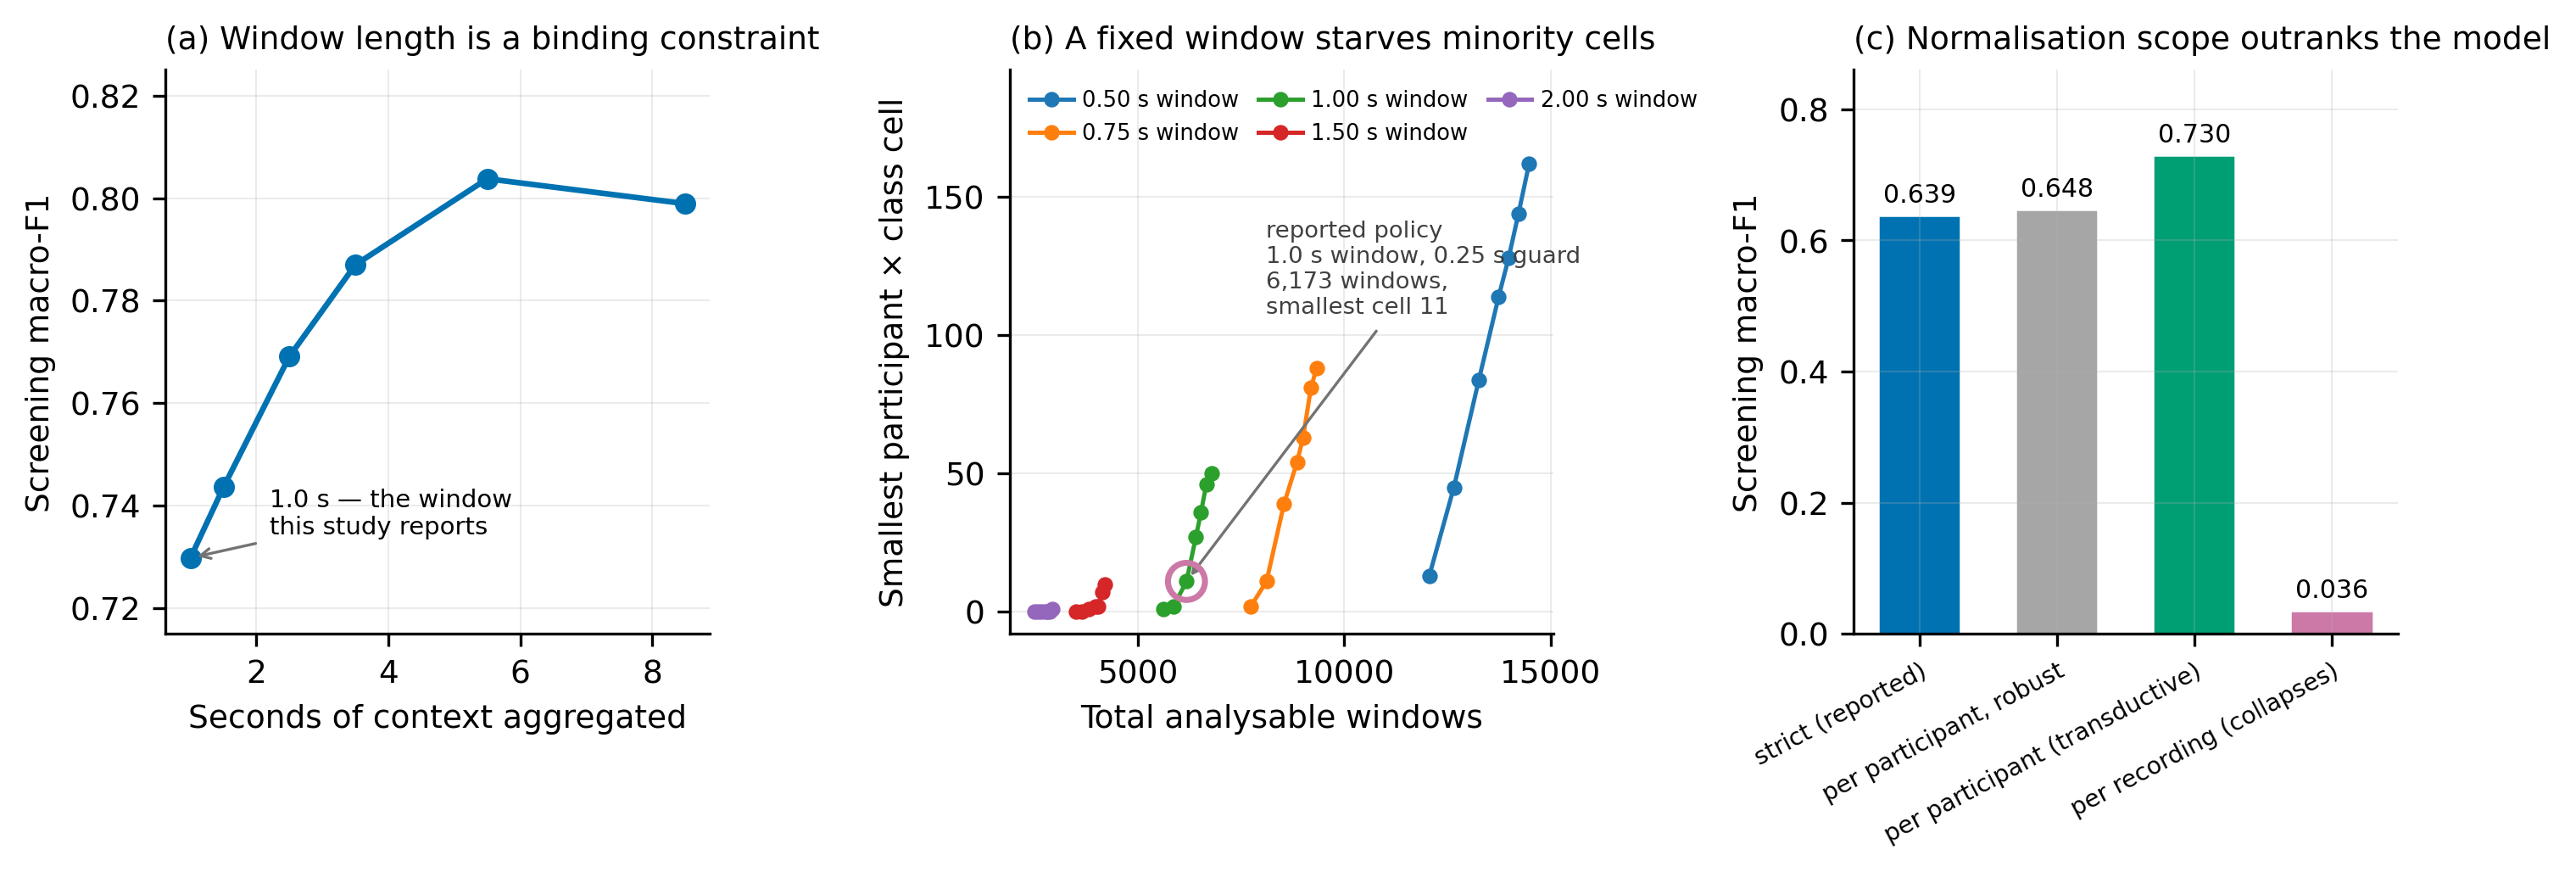
\includegraphics[width=0.74\linewidth]{Figures/v5/design_constraints.png}
  \caption{Three design constraints, measured on identical windows and folds with the screening harness. (a) Macro-F1 against seconds of temporal context aggregated within a recording; monotone across the range, so the 1.0-s window is a constraint rather than a tuned parameter. (b) Every window and guard setting swept: total analysable windows against the smallest participant-and-class cell, reported policy circled. (c) Normalisation scope: the transductive per-participant scope is worth more than the architecture and is used by no reported number.}
  \label{fig:design}
\end{figure*}

\begin{figure*}[t]
  \centering
  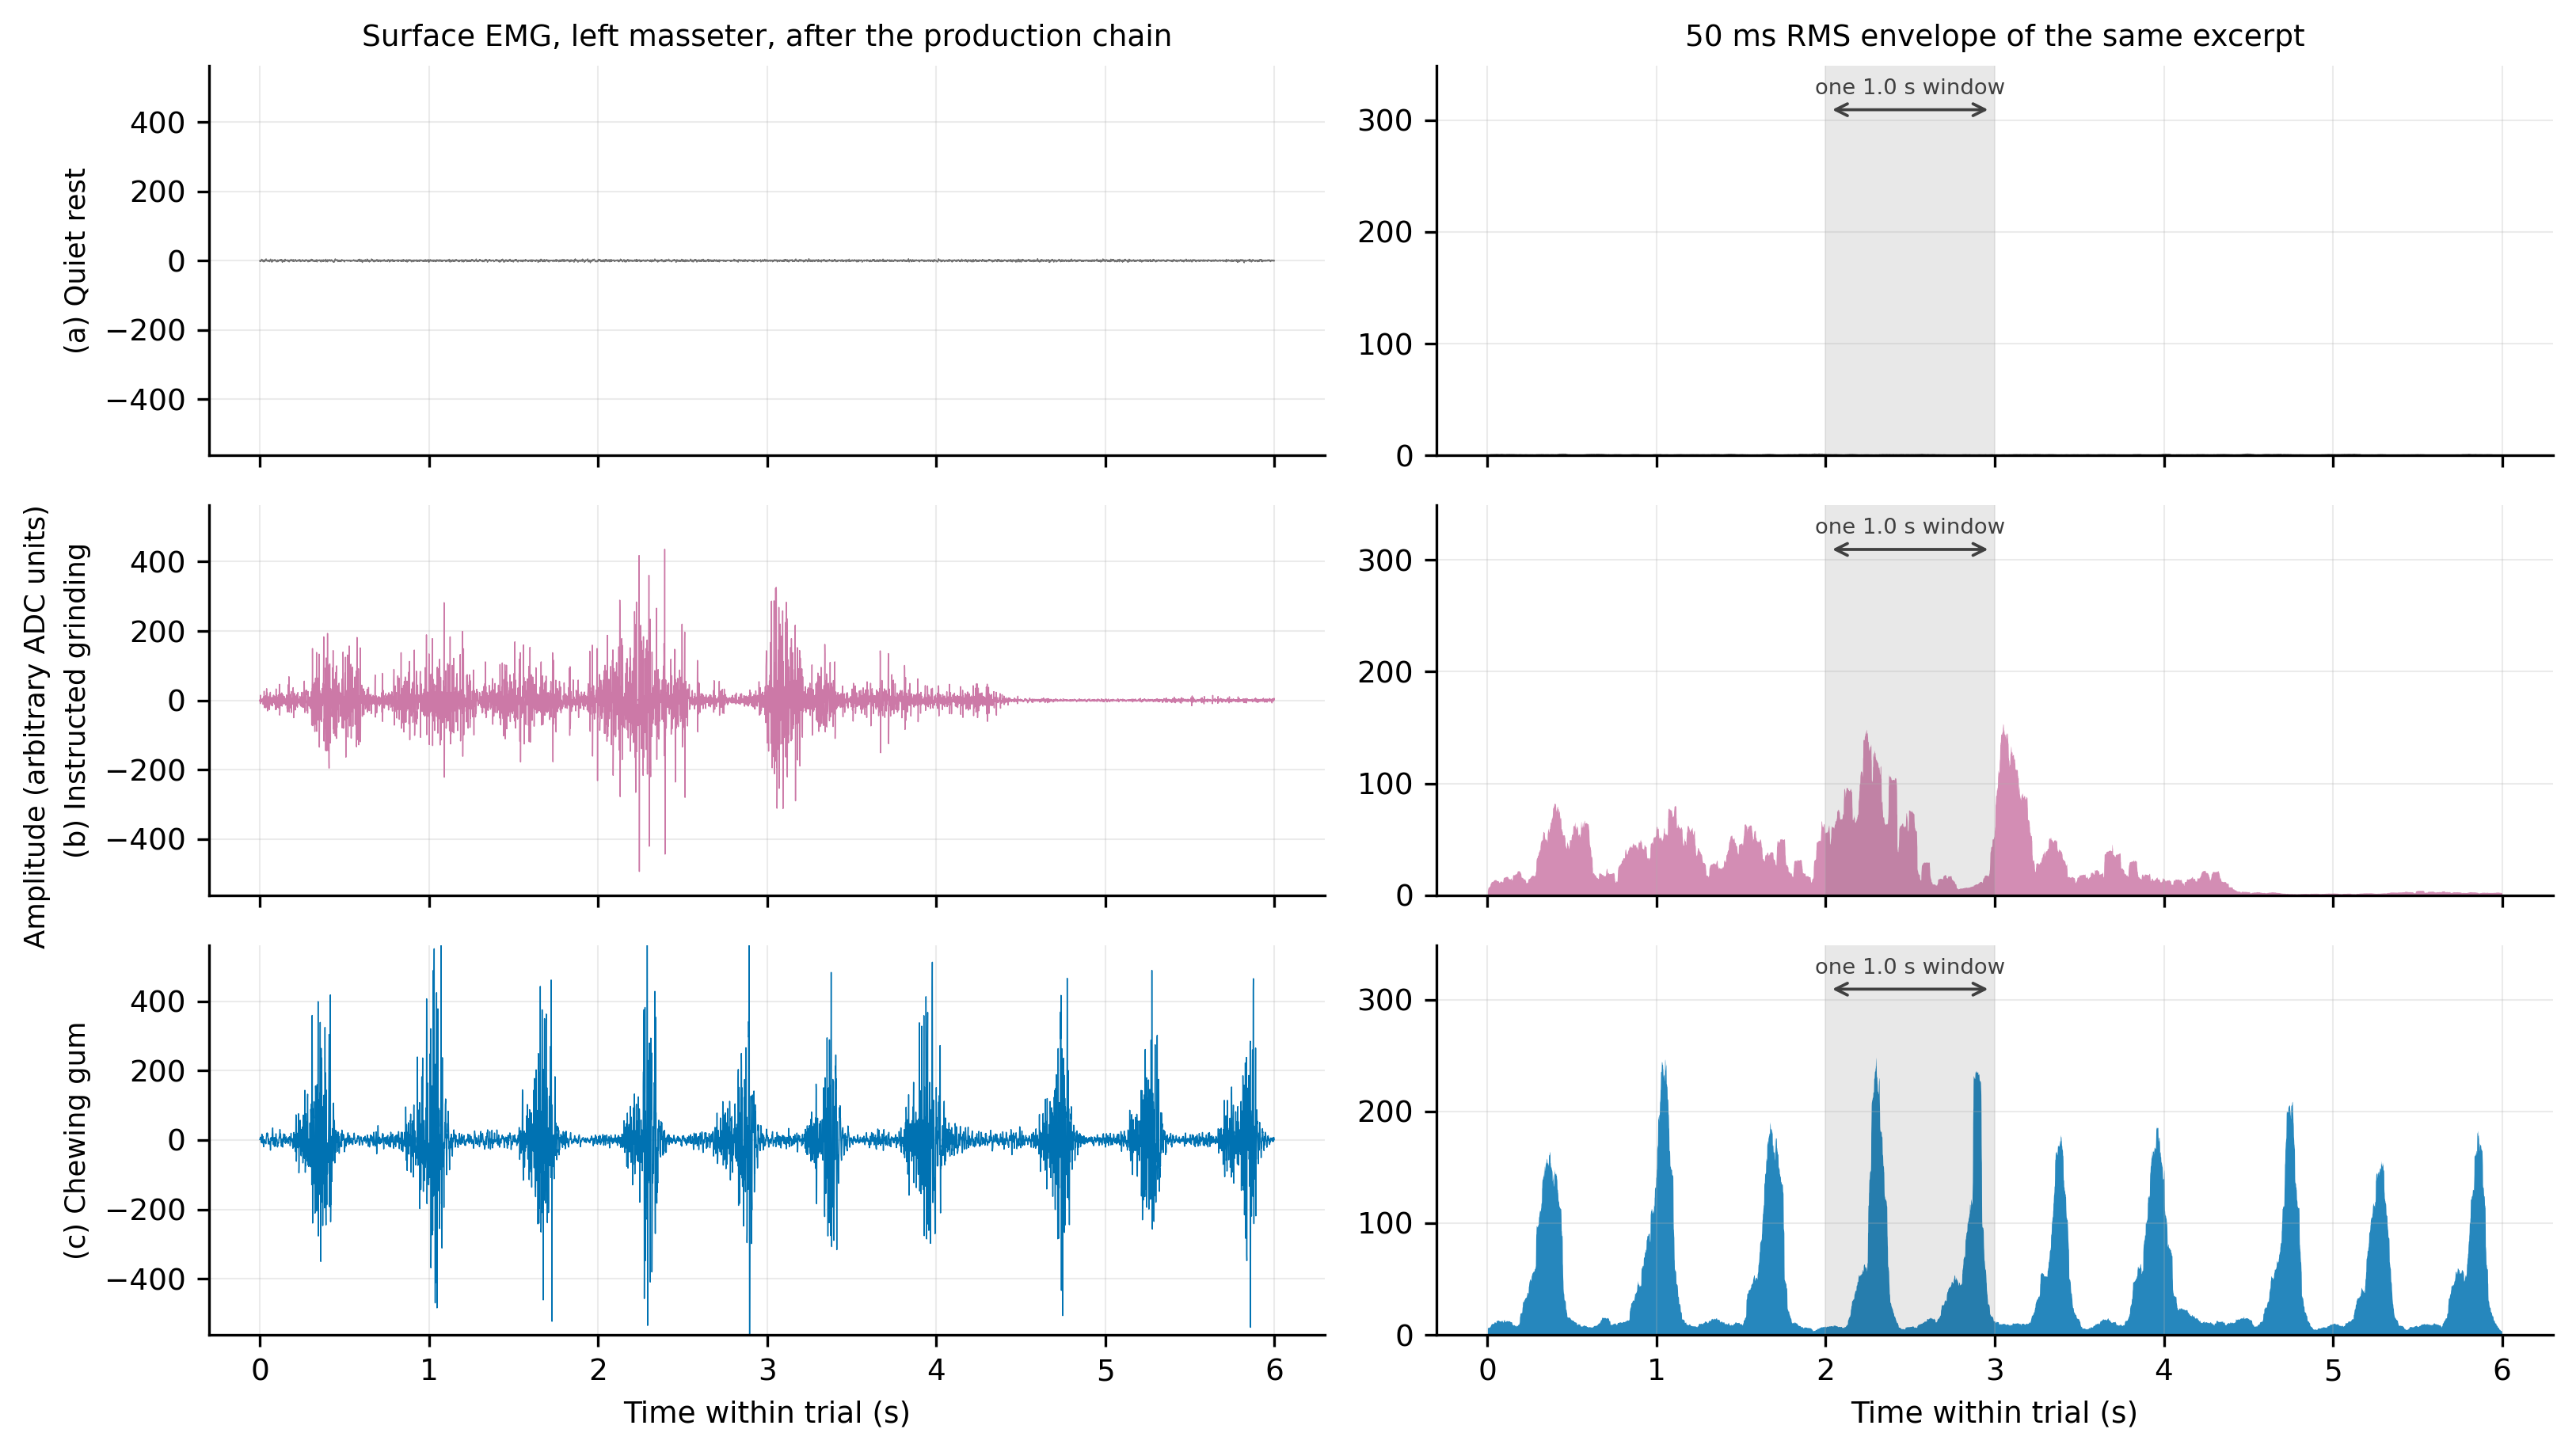
\includegraphics[width=0.62\linewidth]{Figures/v5/signal_comparison_emg.png}
  \caption{Six-second excerpts of one participant's quiet rest, instructed grinding and gum chewing after the corrected chain, on a common scale, with the 50~ms RMS envelope beside each. (a) Rest is quiet. (b) Grinding produces sustained activation without a clear burst and relaxation rhythm. (c) Chewing produces rhythmic bursts at roughly 1.4~Hz. The shaded interval is one 1.0-second analysis window to scale: it holds barely one chewing cycle.}
  \label{fig:signal_comparison}
\end{figure*}

\subsection{Training behaviour and computational cost}
\label{sec:cost}

Because each fold's final model is refit for a fixed epoch budget chosen inside that fold, the curves in Fig.~\ref{fig:loss_curves} are training-fit diagnostics and the held-out participant appears in none of them. Training loss had largely flattened by the end of each budget, and the gap between training-fit and held-out macro-F1 averaged 0.144, largest for P1 at 0.276 and smallest for P5 at 0.040, an ordering that tracks Table~\ref{tab:persubject}: the signature of between-participant variation rather than optimisation failure. Three latencies must be kept separate: the input-context latency of 1000~ms, the window length; the decision interval of 500~ms, the stride; and the processing latency, a median forward pass of 1.02~ms for one window at batch size 1 on an Intel CPU. None supports a wearable or real-time claim: no streaming implementation exists, the production chain is acausal, and power, end-to-end latency and wearable reliability remain unmeasured.

\begin{figure*}[t]
  \centering
  
\includegraphics[width=0.58\linewidth]{Figures/v5/training_curves_5class.png}
  \caption{Refit training loss (a) and training-fit macro-F1 (b) for all fifteen fold and seed combinations, coloured by held-out participant; line style encodes seed. The held-out participant contributes to no curve and is scored once, after training ends.}
  \label{fig:loss_curves}
\end{figure*}

\subsection{What determines performance}
\label{sec:budget}

Table~\ref{tab:budget} collects the six choices priced above on one scale; the ordering is the paper's main result.

Signal quality sets a ceiling that nothing above it can raise. Through the superseded chain the best model scored 43.5\% macro-F1, well below the 61.3\% that the weakest baseline reaches on the corrected signal, so no choice of architecture, features or estimator could have recovered what the filter had passed through untouched. Above that ceiling, what a model can represent matters more than how large it is: the learned wavelet representation beats the band energies it is built from by 8.1 points, an explicit representation of burst and relaxation rhythm gains a further 2.8, and 3.2 times the parameters applied to the raw waveform instead loses 3.3. Two choices fixed before any model was trained fall in the same range or above it, temporal context at 7.4 points and normalisation scope at 9.1, and neither is a modelling decision.

Three cautions apply. The entries are not additive: each is measured against its own baseline, and the temporal-context sweep was run under the per-participant scope, so its 1.0-s starting value of 0.730 is the value that scope earns in the row above it, and adding 7.4 to 9.1 would double-count. The entries do not all come from the same harness: three are confirmatory and three are screening measurements, optimistic in level, so no row should be compared across harnesses to a precision finer than a few points. And the magnitudes are properties of this cohort and this laboratory; what generalises is the ordering and the practice of measuring it.

\begin{table*}[t]
  \centering
  \caption{What determines performance. Six choices priced on the same 6,173 windows and five outer folds, in participant-level macro-F1. The entries are not additive and are not all measured by the same harness (Section~\ref{sec:budget}). ``Reported'' states whether the more favourable setting is the one used for the results in this paper.}
  \label{tab:budget}
  \footnotesize
  \begin{tabular*}{\textwidth}{@{\extracolsep{\fill}}lllrl@{}}
    \toprule
    Choice & Change measured & Harness & $\Delta$ macro F1 & Reported \\
    \midrule
    Signal quality & 60 Hz notch $\rightarrow$ harmonic notch bank & Confirmatory$^{a}$ & $+29.3$ & Yes \\
    Normalisation scope & Strict $\rightarrow$ per-participant & Screening$^{b}$ & $+9.1$ & No$^{c}$ \\
    Learned representation & Band energies $\rightarrow$ wavelet CNN & Conf./screen.$^{d}$ & $+8.1$ & Yes \\
    Temporal context & 1.0 s $\rightarrow$ 5.5 s within a trial & Screening$^{b,e}$ & $+7.4$ & No$^{e}$ \\
    Rhythm representation & Compact $\rightarrow$ extended wavelet CNN & Arch.\ sweep & $+2.8$ & Secondary \\
    Capacity, raw signal & Wavelet CNN $\rightarrow$ early-fusion ($3.2\times$) & Arch.\ sweep & $-3.3$ & No \\
    \bottomrule
  \end{tabular*}
  \begin{flushleft}\footnotesize
  $^{a}$Nested LOSO, three seeds, five outer folds, both arms the fused condition on identical windows, folds and labels (Table~\ref{tab:filter}).
  $^{b}$Screening harness (Section~\ref{sec:screening}): optimistic in level, reliable in direction.
  $^{c}$Excluded by design: it reads the held-out participant's unlabelled feature distribution, which is legitimate, but presumes a per-user fitting session.
  $^{d}$The network is confirmatory and the baseline is screening, so this row crosses harnesses in the conservative direction.
  $^{e}$Trial-level secondary analysis: every recording holds one condition, so aggregation within a recording approaches a majority vote. Its 1.0-s baseline is the per-participant scope of the second row, so these two rows share a baseline and must not be summed.
  \end{flushleft}
\end{table*}

\section{Discussion}

\subsection{What this work contributes}

The first contribution is the analysis and the budget it produced. Table~\ref{tab:budget} places signal quality, learned representation, architecture, temporal context and normalisation scope on one comparable scale, measured on identical windows and folds; to our knowledge no other account in this application area does so, and without one a reported accuracy cannot be attributed to anything. With one, the answer here is unambiguous: fix the signal, then choose what the model can represent, and treat parameter count as the least productive axis of the three.

The second is the dataset and the protocol behind it. Its elements are ordinary; its combination is not, and it was chosen so that every stage of the analysis could later be varied (Section~\ref{sec:why_data}).

The third is the five-class result, and in particular the quiet-rest class: most work in this area classifies activities against each other, which cannot say anything about false alarms, whereas the 7.7\% of rest windows assigned to clenching or grinding here is the closest analogue of a false-alarm rate this design can produce, and the most decision-relevant number in the paper. The fourth is the pipeline taken as a whole, with the signal validated on the way in, the evaluation nested so that model selection cannot see the test participant, three guards that refuse rather than warn, and every number regenerated from a saved prediction ledger: not a novel algorithm, but a working example of an auditable pipeline that another group can copy. The fifth is two checks that cost a single pass over the data: draw the filter response over the measured spectrum of the actual recordings and publish the interference statistic beside the accuracy, and fingerprint every channel of every recording to confirm that no held-out participant's signal appears in its own training set.

\subsection{What the ordering means}

The single sentence we would keep from this study is that what a model can represent mattered more than how large it was, and that signal quality set the ceiling for both.

The architecture sweep makes the first half concrete, because its four models differ mainly in what they are able to see: the two that decompose the signal into wavelet bands placed first and second, the two that do not placed third and fourth, and parameter count ran almost opposite to performance. Within the wavelet pair, the model that could also represent a burst and relaxation rhythm beat the one that could not. That converges with RQ4: the rhythm the extended model can represent within a window is the same information the 1.0-s window withholds, and Section~\ref{sec:constraints} prices access to it at 7.4 points, larger than the 2.8 the architecture recovers by encoding it more cleverly. The binding limitation is informational rather than architectural, and a next study that lengthened the window would likely gain more than one that enlarged the model.

The second half is what RQ1 establishes, and it is easy to overstate. We are not claiming that mains correction is generally worth 29.3 points; in a laboratory with clean recordings it is worth nothing. We are claiming that the ceiling exists, that its height is measurable, and that nothing above it can be interpreted until it has been measured.

\subsection{What transfers beyond this case study}
\label{sec:transfer}

Nothing in the procedure of this paper is specific to EMG or to bruxism, and the procedure should be separated from the numbers it produced here. It has five steps. Audit the signal against what the analysis assumes, on the recordings in hand: draw every filter response over the measured spectrum of the data, fingerprint every channel of every recording, and publish the resulting statistics beside the accuracy. Fix the data, meaning the windows, folds and labels, and vary one stage at a time. Include the choices made before any model was trained, the window length, temporal context, normalisation scope and label source, because here two of them were worth more than the architecture. Report a budget beside the accuracy, naming for each row its harness and its baseline. And keep a prediction ledger from which every number is regenerated.

EEG is the obvious next case, and the pressure points are the same: preprocessing choices there are contested~\cite{delorme2023eeg} and reported inconsistently~\cite{roy2019deep}, architectures are compared under one fixed preprocessing pipeline whose contribution is never priced, and the variance from seeds and splits is often larger than the differences reported between models~\cite{bouthillier2021accounting}. The defect that dominated this study is not an EMG defect either: any electrode-based measurement picks up the mains and its harmonics, any acquisition system may apply filters of its own, and a textbook chain applied on top of them can remove nothing while looking correct.

What does not transfer is the numbers. A laboratory with clean mains would find the first row of Table~\ref{tab:budget} worth nothing; a modality whose informative content is not rhythmic would find temporal context worth less; a task with balanced classes would find normalisation scope worth less. The claim is that the worth of each stage is measurable, that it must be measured before anything above it can be interpreted, and that this holds for every stage between the recording and the reported number.

\subsection{Why signal validation belongs inside the pipeline}

How the defect presented deserves as much attention as its size, because the presentation is what makes it general. It did not look like a signal problem. It looked like between-participant heterogeneity, two of five held-out participants near chance and three in the normal range, which is the most familiar failure mode in this literature and the one that motivates transfer learning, per-user calibration and larger cohorts. A defect in a shared measurement chain expresses itself as apparent variation between the people measured through it, because interference amplitude varies with electrode impedance, cable routing and session rather than with physiology~\cite{deluca2010filtering,besomi2019consensus}, and LOSO attributes that variation to the person held out. It presents as precisely the input-distribution shift that domain generalisation sets out to absorb~\cite{wang2022generalizing,kouw2021review}, and no adaptation could have recovered a signal the filter had passed through untouched. Nothing about the code was wrong: it implemented the filter the literature recommends~\cite{chowdhury2013surface,raez2006techniques}, and its response plot is textbook-correct in isolation. What was missing was one comparison, the filter response drawn over the measured spectrum of the recordings, and one statistic, the share of in-band power within a few hertz of each mains multiple. That is the argument for making validation a stage of the pipeline that can refuse, rather than a review step a careful person performs once.

\subsection{Reading the classification result}

The chewing class deserves a double reading. It supplied most of the windows and achieved the highest F1, and excluding it lowered accuracy while raising macro-F1: a headline accuracy over this class distribution is carried by the easiest and largest class. The clenching and grinding split was retained because clenching is static isometric loading and grinding is lateral excursion under load~\cite{lan2022comparative}, and a system meant to characterise tooth-contact activity should be tested on whether it resolves them; a 1-second window from a grinding bout passing through a static phase may legitimately carry either label, so part of that confusion is label ambiguity rather than model error. Comparison with the greater-than-90\% accuracy of Sonmezocak and Kurt~\cite{sonmezocak2021detection} is not like-for-like: their classes differ, their segments from ten volunteers were split at random rather than held out by participant, and dataset composition, preprocessing and sample size all differ (Table~\ref{tab:positioning}).

\subsection{What a next study should do}

Section~\ref{sec:constraints} priced three choices this design fixed early, and two proved worth more than the architecture. Temporal context is the clearest: performance rises monotonically from 1.0 to 5.5~s, so the 1-second window is a limitation of this analysis rather than an optimum it found; a next design should aggregate over a declared context and evaluate on continuously varying activity. Trigger granularity is the least obvious constraint and the easiest to fix: because participants marked bouts as they saw fit, one produced seven times as many clenching windows as another from the same task, an instruction problem removable by standardising trigger use. Normalisation scope is a product decision disguised as a preprocessing one: standardising by the held-out participant's own unlabelled distribution is legitimate but presumes a per-user fitting session, and the strict scope is reported because it supports the more defensible claim~\cite{besomi2020consensus}.

Setting is the remaining gap. Laboratory repetitions do not capture the frequency, duration or variability of behaviour outside the laboratory; awake bruxism is currently characterised mainly by ecological momentary assessment~\cite{bracci2018frequency}. A next-stage awake study should combine multi-day EMG with a clearly defined background class and blinded annotation of candidate episodes, and report false positives per hour. No conclusion about sleep follows from these awake tasks; a sleep study would require overnight data, sleep staging, comparison with polysomnography or validated portable assessment, and repeated nights~\cite{lavigne1996sleep,casett2017validity,cidverdejo2024instrumental}.

\subsection{Validity and limitations}

The principal limitation is the cohort size, at $N=5$. The 6,173 overlapping windows supply many optimisation examples but do not replace independent participants: adjacent windows share half their samples and one participant contributed 27\% of them. LOSO does not establish external generalisation from five people~\cite{varoquaux2018cross}. The budget of Table~\ref{tab:budget} inherits that limitation: its entries are not additive and share a baseline in one place, and three of its six rows are screening measurements, optimistic in level. It should be read as an ordering with approximate magnitudes, not as a decomposition of variance.

The RQ1 contrast comes from one cohort in one laboratory, and its magnitude is not a general effect size. Two features bound it in opposite directions: the superseded arm carried an extra input channel and searched its hyperparameters, making the gap conservative; but the two runs differ in codebase version, and although the windows, folds and labels are byte-identical and were verified as such, an unrecorded contributing difference cannot be excluded.

Task coverage and label precision bound what the classes mean. The tasks cover tooth-contact clenching and grinding but not bracing or thrusting~\cite{verhoeff2025definitions}, and the prior diagnoses were not phenotyped~\cite{manfredini2024standardised}. Class membership rests on a button press: muscle activity preceded the marker at four of every five onsets, and although the 0.25-s guard covers the 95th percentile of the harmful direction, some trial-leading windows may carry a partially mislabelled edge. Instructed activity may be more regular, longer or more forceful than spontaneous activity, a bias in the optimistic direction~\cite{farella2008masticatory}. Rest was recorded in a controlled laboratory and did not sample speaking, swallowing, facial expression, head movement or other free-living behaviour, so the analysis can estimate confusion against quiet rest but not false alarms per hour during unrestricted use.

Two limitations belong to the framing. Table~\ref{tab:positioning} is a comparison, not a systematic review: its entries were checked against the sources, but the search was not exhaustive, and an unreported check is not proof of an absent one. And the generality claimed in Section~\ref{sec:transfer} is for the procedure, carried out once, on one modality, in one laboratory; whether the ordering recurs elsewhere is a question this study poses and does not answer.

\section{Conclusion}

This study asked, of one biosignal classification pipeline, where its performance comes from, and answered by measurement: each stage was varied while the windows, folds and labels were held fixed, and the effects were placed on one scale. On participants it had never seen, the pipeline separated quiet rest and four instructed jaw activities from surface EMG at 81.7\% accuracy and 72.0\% macro-F1 in 5,901 parameters, with quiet rest the best-recalled class.

The ordering is the more durable result. Signal quality set a ceiling: correcting a mains-harmonic defect that the conventional chain had left untouched moved the matched network by 29.3 points of macro-F1 on identical windows, folds and labels. Above that ceiling, what a model could represent mattered more than its size: the two architectures that decomposed the signal into wavelet bands placed above the two that did not, and the largest of the four placed third. Two choices fixed before any model was trained, temporal context and normalisation scope, were each worth as much as the architecture or more. The transferable recommendation costs one pass over the data: report a measured interference statistic beside every accuracy, draw filter responses over the measured spectrum of the recordings rather than alone, and fingerprint every channel of every recording to confirm that no held-out participant's signal appears in its own training set.

This study does not validate a bruxism detection device: there is no bracing or thrusting, no unrestricted background behaviour, no spontaneous episode, no sleep recording and no independent reference standard. The defensible conclusion for the case study is that surface EMG with a wavelet representation merits further evaluation in a larger, phenotyped, multi-day study. The defensible conclusion for the field is broader. Between a recording and a reported accuracy sit half a dozen stages, each of which can be worth more than the model and each of which can be priced with the data already in hand. A paper that publishes that budget beside its accuracy, for EEG, ECG or inertial signals as much as for EMG, tells its readers what to copy; a paper that publishes the accuracy alone does not.

\backmatter

\section*{Data availability}
The datasets generated and analysed during the current study are not publicly available because of participant-privacy restrictions but are available from the corresponding author on reasonable request, subject to institutional and ethical requirements. The archive holds, per recording, the six-column file as acquired, its metadata sidecar and the review video; the videos are identifiable and are not shared.

\section*{Code availability}
The custom code for preprocessing, wavelet decomposition, training and evaluation is available from the corresponding author on reasonable request. Every number and figure was regenerated from a saved artifact. The confirmatory five-class results come from the EMG conditions of run \texttt{modality\_and\_no\_chewing\_}\allowbreak\texttt{20260810T020642\_cead62e4} (configuration hash \texttt{cead62e4}, manifest \texttt{7ebbcc8d}, window index \texttt{b2cf690c}); the architecture sweep from run \texttt{baselines\_emg\_only\_20260816} (manifest \texttt{9d93667b}, window index \texttt{9941fe48}); comparing the two prediction ledgers window by window returns the identical 6,173 windows, labels and held-out assignments. Parameter counts and latencies come from \texttt{outputs/benchmarks/}\allowbreak\texttt{benchmark\_emg\_only.json}.

\section*{Funding declaration}
Research reported in this publication was supported by an award from the Rhode Island Life Science Hub Small Grant Program (Principal Investigator T. A. Walls; Co-Investigators R. Abiri and M. Furmanek). The project was also partially supported by National Science Foundation grant 2245558 (Principal Investigator R. Abiri).

\section*{Acknowledgements}
We thank University of Rhode Island undergraduate and graduate students Anjolaoluwa Akingbile, Jessica Constantine and Nathan DeSalvo, who located and summarised the functions of bruxism devices before this project.

\section*{Author contributions}
M.H.F.: methodology, software, analysis, writing---original draft, and writing---review and editing. A.R.: protocol development, software, data curation, data collection, formal analysis, and review and editing. R.S.: methodology, validation, and writing---review and editing. M.P.F.: conceptualization and study design, research-grant development, protocol development, and manuscript revision. R.A.: conceptualization, project administration, resources, supervision, and writing---review and editing. T.A.W.: conceptualization, research-grant authorship, protocol development, project oversight, and manuscript revision. All authors reviewed and approved the final manuscript.

\section*{Competing interests}
The authors declare no competing interests.

\bibliography{refs_v8}

\end{document}
